% ---------------------------------------------------------------------------------------------------------------
% TEMPLATE PARA TRABALHO DE CONCLUSÃO DE CURSO
% Universidade Tecnológica Federal do Paraná - UTFPR
% Customização da classe abnTeX2 (http://www.abntex.net.br/) para as normas da UTFPR
%
% Projeto hospedado em: <link git>
% Autores: Diego Marczal  <>
% 	   Michael Vornes <https://github.com/mvornes>
%
%----------------------------------------------------------------------------------------------------------------
% Codificação: UTF-8
% LaTeX:  abnTeX2          
% ---------------------------------------------------------------------------------------------------------------


% CARREGA CLASSE PERSONALIZADA DA UTFPR--------------------------------------------------------------------------
\documentclass[%twoside,                   % Impressão em frente e verso
    	        oneside,                   % Impressão apenas frente
]{configuracoes/utfpr-abntex2}


% INCLUI ARQUIVOS DE CONFIGURAÇÕES-------------------------------------------------------------------------------
% REFERÊNCIAS------------------------------------------------------------------
\usepackage[%
    alf,
    abnt-emphasize=bf,
    bibjustif,
    recuo=0cm,
    abnt-url-package=url,       % Utiliza o pacote url
    abnt-refinfo=yes,           % Utiliza o estilo bibliográfico abnt-refinfo
    abnt-etal-cite=3,
    abnt-etal-list=3,
    abnt-thesis-year=final
]{abntex2cite}                  % Configura as citações bibliográficas conforme a norma ABNT

% PACOTES----------------------------------------------------------------------
\usepackage[utf8]{inputenc}                                 % Codificação do documento
\usepackage[T1]{fontenc}                                    % Seleção de código de fonte
\usepackage{booktabs}                                       % Réguas horizontais em tabelas
\usepackage{color, colortbl}                                % Controle das cores
\usepackage{float}                                          % Necessário para tabelas/figuras em ambiente multi-colunas
\usepackage{graphicx}                                       % Inclusão de gráficos e figuras
\usepackage{icomma}                                         % Uso de vírgulas em expressões matemáticas
\usepackage{indentfirst}                                    % Indenta o primeiro parágrafo de cada seção
\usepackage{microtype}                                      % Melhora a justificação do documento
\usepackage{multirow, array}                                % Permite tabelas com múltiplas linhas e colunas
\usepackage{subeqnarray}                                    % Permite subnumeração de equações
\usepackage{lastpage}                                       % Para encontrar última página do documento
\usepackage{verbatim}                                       % Permite apresentar texto tal como escrito no documento, ainda que sejam comandos Latex
\usepackage{amsfonts, amssymb, amsmath}                     % Fontes e símbolos matemáticos
\usepackage[algoruled, portuguese]{algorithm2e}             % Permite escrever algoritmos em português
%\usepackage[scaled]{helvet}                                % Usa a fonte Helvetica
\usepackage{times}                                          % Usa a fonte Times
%\usepackage{mathptmx}
%\usepackage{palatino}                                      % Usa a fonte Palatino
%\usepackage{lmodern}                                       % Usa a fonte Latin Modern
\usepackage[bottom]{footmisc}                               % Mantém as notas de rodapé sempre na mesma posição
\usepackage{ae, aecompl}                                    % Fontes de alta qualidade
\usepackage{latexsym}                                       % Símbolos matemáticos
\usepackage{lscape}                                         % Permite páginas em modo "paisagem"
%\usepackage{picinpar}                                      % Dispor imagens em parágrafos
%\usepackage{scalefnt}                                      % Permite redimensionar tamanho da fonte
%\usepackage{subfig}                                        % Posicionamento de figuras
%\usepackage{upgreek}                                       % Fonte letras gregas


% Redefine a fonte para uma fonte similar a Arial (fonte Helvetica)
\renewcommand*\familydefault{\sfdefault}

% CONFIGURAÇÕES DE APARÊNCIA DO PDF FINAL--------------------------------------
\makeatletter
\hypersetup{%
    portuguese,
    colorlinks=true,   % true: "links" coloridos; false: "links" em caixas de texto
    linkcolor=blue,    % Define cor dos "links" internos
    citecolor=blue,    % Define cor dos "links" para as referências bibliográficas
    filecolor=blue,    % Define cor dos "links" para arquivos
    urlcolor=blue,     % Define a cor dos "hiperlinks"
    breaklinks=true,
    pdftitle={\@title},
    pdfauthor={\@author},
    pdfkeywords={abnt, latex, abntex, abntex2}
}
\makeatother

% ALTERA O ASPECTO DA COR AZUL--------------------------------------------------
\definecolor{blue}{RGB}{41,5,195}

% REDEFINIÇÃO DE LABELS---------------------------------------------------------
\renewcommand{\algorithmautorefname}{Algoritmo}
\def\equationautorefname~#1\null{Equa\c c\~ao~(#1)\null}

% CRIA ÍNDICE REMISSIVO---------------------------------------------------------
\makeindex

% HIFENIZAÇÃO DE PALAVRAS QUE NÃO ESTÃO NO DICIONÁRIO---------------------------
\hyphenation{%
    qua-dros-cha-ve
    Kat-sa-gge-los
}



% INCLUI ARQUIVOS DO TRABALHO DE CONCLUSÃO DE CURSO (PRÉ-TEXTUAIS, TEXTUAIS, PÓS-TEXTUAIS)-----------------------

% INSERE CAPA E FOLHA DE ROSTO
% CAPA---------------------------------------------------------------------------------------------------

% ORIENTAÇÕES GERAIS-------------------------------------------------------------------------------------
% Caso algum dos campos não se aplique ao seu trabalho, como por exemplo,
% se não houve coorientador, apenas deixe vazio.
% Exemplos: 
% \coorientador{}
% \departamento{}

% DADOS DO TRABALHO--------------------------------------------------------------------------------------
\titulo{FishSpot: Encontre o melhor lugar para pescar }
\titleabstract{FishSpot: Find the best place to fish }
\autor{Gabriel Alves de Moura}
\autorcitacao{MOURA, Gabriel}
\local{Itapetininga}
\data{2025}

% NATUREZA DO TRABALHO-----------------------------------------------------------------------------------
% Opções: 
% - Trabalho de Conclusão de Curso (se for Graduação)
% - Dissertação (se for Mestrado)
% - Tese (se for Doutorado)
% - Projeto de Qualificação (se for Mestrado ou Doutorado)
\projeto{Trabalho de Conclusão de Curso}

% TÍTULO ACADÊMICO---------------------------------------------------------------------------------------
% Opções:
% - Bacharel ou Tecnólogo (Se a natureza for Trabalho de Conclusão de Curso)
% - Mestre (Se a natureza for Dissertação)
% - Doutor (Se a natureza for Tese)
% - Mestre ou Doutor (Se a natureza for Projeto de Qualificação)
\tituloAcademico{Especialista}

% ÁREA DE CONCENTRAÇÃO E LINHA DE PESQUISA---------------------------------------------------------------
% Se a natureza for Trabalho de Conclusão de Curso, deixe ambos os campos vazios
% Se for programa de Pós-graduação, indique a área de concentração e a linha de pesquisa
\areaconcentracao{Informática Aplicada a Educação}
%\linhapesquisa{Uso de plataformas digitais baseada em jogos no auxilio do processo ensino aprendizagem}

% DADOS DA INSTITUIÇÃO-----------------------------------------------------------------------------------
% Se a natureza for Trabalho de Conclusão de Curso, coloque o nome do curso de graduação em "programa"
% Formato para o logo da Instituição: \logoinstituicao{<escala>}{<caminho/nome do arquivo>}
\instituicao{Instituto Federal de Educação, Ciência e Tecnologia de São Paulo}
\departamento{Campus Itapetininga}
\programa{curso de Pós Graduação em Informática Aplicada a Educação}
\logoinstituicao{0.2}{dados/figuras/logo-instituicao.png} 

% DADOS DOS ORIENTADORES---------------------------------------------------------------------------------
\orientador{Anderson Bernardo de Almeida}
\instOrientador{}

%\coorientador{Nome do coorientador}
%\coorientador[Coorientadora:]{Nome da coorientadora}
%\instCoorientador{Instituição do coorientador}

% FOLHA DE ROSTO--------------------------------------------------------------------------------------------------------

% TRABALHO DE CONCLUSÃO DE CURSO
 \preambulo{{\imprimirprojeto} apresentado ao {\imprimirinstituicao}, {\imprimirdepartamento}, como requisito para a obtenção do título de {\imprimirtituloAcademico} em {\imprimirareaconcentracao}.}

% DISSERTAÇÃO DE MESTRADO
% \preambulo{{\imprimirprojeto} apresentada ao Programa de \mbox{Pós-graduação} do {\imprimirinstituicao}, como requisito parcial para obtenção do título de {\imprimirtituloAcademico}.}

% TESE DE DOUTORADO
% \preambulo{{\imprimirprojeto} apresentada ao Programa de \mbox{Pós-graduação} da {\imprimirinstituicao}, como requisito parcial para a obtenção do título de {\imprimirtituloAcademico}.}

% PROJETO DE QUALIFICAÇÃO DE MESTRADO OU DOUTORADO
%\preambulo{{\imprimirprojeto} apresentado ao Programa de \mbox{Pós-graduação} da {\imprimirinstituicao}, como requisito parcial para a obtenção do título de {\imprimirtituloAcademico}.}

% OBSERVAÇÕES-----------------------------------------------------------------------------------------------------------
% Altere este arquivo APENAS comentando as linhas que não se aplicam ao tipo de trabalho acadêmico desejado.



\begin{document}

\pretextual
\imprimircapa                                               	       % Comando para imprimir Capa
\imprimirfolhaderosto{}                                     		   % Comando para imprimir Folha de rosto

% INSERE ELEMENTOS PRÉ-TEXTUAIS
% -----------------------------------------------------------------------------
% Folha de Aprovação
% -----------------------------------------------------------------------------

\begin{folhadeaprovacao}

  \begin{center}
    {\ABNTEXchapterfont\large\MakeUppercase{\imprimirautor}}

    \vspace*{\fill}\vspace*{\fill}
    \begin{center}
      \ABNTEXchapterfont\bfseries\Large\MakeUppercase{\imprimirtitulo}
    \end{center}
    \vspace*{\fill}
     
    \vspace*{1cm}
    
	\imprimirlocal, X de Y de 2025:

    \vspace*{\fill}

   \end{center}
        


   \assinatura{\textbf{\imprimirorientador, Dr.} \\ Orientador\\Instituto Federal de São Paulo} 
   \assinatura{\textbf{Professor, Dr.} \\ Instituto X }
   \assinatura{\textbf{Professor} \\ Instituto Y}
   \assinatura{\textbf{Professor} \\ Instituto Z}
   %\assinatura{\textbf{Professor} \\ Convidado 4}
      
    \vspace*{1cm}  
  
\end{folhadeaprovacao}

% -----------------------------------------------------------------------------
% Este documento foi mantido apenas para preservar a paginação do trabalho
% acadêmico final, após a inserção da folha de aprovação fornecida
% -----------------------------------------------------------------------------

%% DEDICATÓRIA------------------------------------------------------------------

\renewcommand{\dedicatorianame}{DEDICATÓRIA}

\begin{dedicatoria}

Escrever a dedicatoria aqui

\end{dedicatoria}
          			             % Dedicatória
%% AGRADECIMENTOS---------------------------------------------------------------

\begin{agradecimentos}[AGRADECIMENTOS]

Escrever agradecimentos aqui

\end{agradecimentos}
        			         % Agradecimentos
% EPÍGRAFE---------------------------------------------------------------------

\renewcommand{\epigraphname}{EPÍGRAFE}

\begin{epigrafe}

\textit{"Se você quer transformar o mundo, experimente primeiro promover o seu aperfeiçoamento pessoal e realizar inovações no seu próprio interior.", Dalai Lama.}

\end{epigrafe}

% OBSERVAÇÕES------------------------------------------------------------------
% Altere o texto para inserir a epígrafe do seu trabalho

              			             % Epígrafe
% RESUMO--------------------------------------------------------------------------------

\begin{resumo}[RESUMO]
\begin{SingleSpacing}

% Auto citação completa--------------------------------------------------------
%\imprimirautorcitacao. \imprimirtitulo. \imprimirdata. \pageref {LastPage} f. \imprimirprojeto\ – %\imprimirprograma, \imprimirinstituicao. \imprimirlocal, \imprimirdata.\\
%---------------------------------------------------------------------------------------


\hfill \break
\textbf{Palavras-chave}: Pesca. Plataforma Digital. Aplicação Móvel. Software, Desenvolvimento.

\end{SingleSpacing}
\end{resumo}

% OBSERVAÇÕES---------------------------------------------------------------------------
% Altere o texto inserindo o Resumo do seu trabalho.
% Escolha de 3 a 5 palavras ou termos que descrevam bem o seu trabalho 

             			             % Resumo em Português
% ABSTRACT--------------------------------------------------------------------------------

\begin{resumo}[ABSTRACT]
\begin{SingleSpacing}

% Auto-Citação completa em Ingles--------------------------------------------------------
%\imprimirautorcitacao. \imprimirtitleabstract. \imprimirdata. \pageref {LastPage} f. \imprimirprojeto\ – %\imprimirprograma, \imprimirinstituicao. \imprimirlocal, \imprimirdata.\\
%---------------------------------------------------------------------------------------

\textbf{Keywords}: .
\end{SingleSpacing}
\end{resumo}

% OBSERVAÇÕES---------------------------------------------------------------------------
% Altere o texto inserindo o Abstract do seu trabalho.
% Escolha de 3 a 5 palavras ou termos que descrevam bem o seu trabalho 
             		                 % Resumo em Inglês
% Lista de Figuras----------------------------------------------------------------

\hypersetup{linkcolor = black}
\pdfbookmark[0]{\listfigurename}{lof}
\listoffigures*
\cleardoublepage

% OBSERVAÇÕES---------------------------------------------------------------------
% Este arquivo não precisa de ser alterado, pois a lista é gerada automaticamente.
                        % Lista de Figuras
%\include{estrutura/pre-textuais/listas/listas-ilustracoes/lista-quadros}    % Lista de Quadros
% LISTA DE TABELAS-------------------------------------------------------------

\pdfbookmark[0]{\listtablename}{lot}
\listoftables*
\cleardoublepage

% OBSERVAÇÕES-------------------------------------------------------------------
% Este arquivo não precisa ser alterado, pois a lista é gerada automaticamente.
         		         % Lista de Tabelas
% LISTA DE ABREVIATURAS E SIGLAS----------------------------------------------------------

\begin{siglas}
    \item[IFSP] Instituto Federal de São Paulo
    \item[API] Application Programming Interface
    \item[JSON] JavaScript Object Notation
    \item[UX] User Experience
    \item[OSM] OpenStreetMap 
\end{siglas}

% OBSERVAÇÕES-----------------------------------------------------------------------------
% Altere a lista acima para definir os acrônimos e siglas utilizados neste trabalho
          		         % Lista de Abreviaturas e Siglas
%\include{estrutura/pre-textuais/listas/lista-simbolos}        		         % Lista de Símbolos
%\include{estrutura/pre-textuais/listas/listas-diversas/lista-algoritmos}    % Lista de Algoritmos
% SUMÁRIO----------------------------------------------------------------------

\renewcommand{\contentsname}{SUMÁRIO}

\pdfbookmark[0]{\contentsname}{toc}
{
    \hypersetup{linkcolor=black}
    \tableofcontents*
}
\cleardoublepage

% OBSERVAÇÕES-------------------------------------------------------------------
% Este arquivo não precisa ser alterado, pois o sumário é gerado automaticamente.
               			             % Sumário

\textual
% INSERE ELEMENTOS TEXTUAIS
% INTRODUÇÃO-------------------------------------------------------------------

\chapter{INTRODUÇÃO}
\label{chap:introducao}

%O trabalho será desenvolvido com o intuito de cobrir uma parte dos pescadores que possuem dificuldades em localizar bons locais de pesca, sejam eles em lugares remotos ou até mesmo em pesqueiros. O aplicativo terá como objetivo principal a disponibilização de um mapa onde será possível realizar a visualização dos pontos de pescas registrados por outros usuários.

% A partir de um breve levantamento qualitativo de dados realizados com pescadores, percebe-se que muitos sofrem para encontrar um rio, uma lagoa ou até mesmo um pesqueiro adequado para que tenham um tempo de lazer, tendo em vista que esse processo pode levar de horas ou até mesmo dias.  

% A existência de um aplicativo que possui tal funcionalidade é clara, entretanto a inexistência do próprio traduzido em português pode levar os usuários a não utilizarem as funcionalidades de registro e visualização dos peixes e locais de pesca devido à maioria não possuir conhecimento na língua inglesa.


                		          % Introdução
\chapter{JUSTIFICATIVA}
\label{chap:justificativa}

Atualmente, é comum a utilização de aplicativos para o preparo de uma rotina de pesca. A facilidade de encontrar locais de pescaria, bem como a visualização de detalhes sobre os peixes presentes e as iscas utilizadas, trazem segurança e tranquilidade para o cotidiano de um pescador.

Embora existam várias aplicações com esse propósito, é raro possuírem experiência de usuário (UX, \textit{User Experience}) de acordo com as necessidades do usuário comum. Frequentemente disponíveis sem tradução completa para a língua portuguesa, bem como faltando simplicidade em sua interface, o uso das ferramentas que buscam ser compreensíveis se torna algo complexo, de difícil aprendizado, impedindo o desfruto de momentos de lazer proporcionados pela pesca ao pescador.

Dessa forma, este aplicativo busca apoiar a colaboração da comunidade de pescadores para aumentar a eficiência durante o processo, permitindo que os usuários registrem os locais visitados, as dificuldades enfrentadas para chegar até esses pontos, os riscos encontrados durante a pesca e as espécies de peixes capturadas no período de lazer de forma fácil e compreensível, eliminando as dificuldades decorrentes de uma interface confusa e proporcionando aos usuários uma experiência tranquila e acessível.

O objetivo final desse projeto é proporcionar aos membros mais agilidade e simplicidade na busca por locais ideais, reduzindo o tempo necessário na pesquisa e, assim, trazendo maior eficácia na captura de bons exemplares de peixes e mais segurança durante todo o processo.

% ---

                            % Justificativa
% OBJETIVOS------------------------------------------------------------------

\chapter{OBJETIVOS}
\label{chap:objetivos}

\section{OBJETIVOS GERAIS}
\label{sec:objetivosGerais}

O objetivo geral deste trabalho é criar uma aplicação móvel que auxilie pescadores na identificação e localização de pontos de pesca, visando otimizar o processo de busca, aumentar a eficiência nas atividades e melhorar a experiência do usuário.

\section{OBJETIVOS ESPECÍFICOS}
\label{sec:objetivosEspecificos}

\begin{itemize}
  \item Registrar dados que descrevam quais foram os resultados obtidos após a pesca através de um formulário simples;
  \item Mostrar pontos de pesca em um mapa, semelhante aos pontos de referências usados por aplicativos de geolocalização como Google Maps, Waze, Uber e entre outros;
  \item Detalhar dados obtidos por pescadores para todos os membros da plataforma;
  \item Gerenciar dados registrados na aplicação, dentre eles dados sigilosos ou informações sobre os pontos de pesca;
  \item Trazer os sentimentos de liberdade, tranquilidade, paz e conforto para o pescador através das cores utilizadas no design da aplicação;
  \item Criar uma aplicação acessível, onde os usuários sejam capazes de utilizar mesmo que possuam limitações;
  \item Assegurar a compreensão clara de todas as funcionalidades da aplicação, mantendo uma ótima experiência de usuário. 
\end{itemize}                                % Objetivos

% METODOLOGIA------------------------------------------------------------

\chapter{METODOLOGIA}
\label{chap:metodologia}

O presente trabalho é considerado uma pesquisa de natureza aplicada, pois procura, através da análise de alguns recursos, desenvolver o conhecimento para aplicar uma solução para o problema apontado neste documento.

Considerando seus objetivos, o presente documento se caracteriza como uma pesquisa descritiva e exploratória, pois utilizará fontes acadêmicas para ser fundamentada e também busca sondar o problema descrito neste documento por meio de formulários e entrevistas com a comunidade.

Quanto à forma de abordagem, este projeto se enquadra em pesquisa qualitativa, pois como abordado por \citeonline{godoy1995introduccao}, o que é valorizado na pesquisa qualitativa é o contato direto e prolongado do pesquisador com o ambiente e situação que está sendo estudada, e também descreve que um fenômeno pode ser bem mais observado e compreendido no contexto em que ocorre. Desse modo a pesquisa poderá identificar não só a dificuldade que os pescadores possuem ao encontrar um local de pesca, mas também as formas e meios utilizados para localizar um bom local longe de perigos.

O tipo de procedimento técnico utilizado para este trabalho será levantamento, pois de acordo com o \citeonline{de2023metodologia} a pesquisa de levantamento é uma estratégia utilizada para levantar dados e informações sobre características ou opiniões de um grupo. Contudo, devido à necessidade da leitura de documentos para assegurar que as informações levantadas estão de fato pautadas em verdade, esta pesquisa conta com um âmbito documental.

\section{COLETA E TRATAMENTO DE DADOS}
\label{sec:titSecColDad}

A principal forma de coleta de dados será por meio de formulários e questionários, que permitirão reunir informações de forma estruturada e padronizada. Os formulários poderão ser físicos ou digitais, facilitando a coleta em larga escala e garantindo uniformidade nas respostas, enquanto os questionários serão mais detalhados, abordando questões específicas relacionadas ao tema da pesquisa.

Os formulários serão utilizados em locais com grande fluxo de pessoas, como pesqueiros, parques os quais possuem tanques de pesca e locais de acampamento com lagos, desta forma facilitando a coleta dos dados. Os questionários serão utilizados em locais onde perguntas mais detalhadas devem ser feitas, como exemplo rios e lagos localizados longe do perímetro urbano, córregos que possuem tratamento e a vida nativa é saudável, praias, pescas em alto-mar e dentre outros locais de pesca.

A análise dos resultados obtidos nos questionários será executada de forma qualitativa, e poderá ser identificado quais são as dificuldades encontradas durante o processo de localização do melhor local de pesca.
                              % Metodologia
% REFERENCIAL TEORICO----------------------------------------------------

\chapter{REFERENCIAL TEÓRICO}
\label{chap:referencialTeorico}

\section{TECNOLOGIA NA PESCA}
\label{sec:referenciasDeDesenvolvimento}

\citeonline{afonso2007breves} destaca que a pesca surgiu como uma prática adotada pelos seres humanos para obter alimento. Com o passar do tempo, essa atividade tornou-se mais eficiente, graças ao desenvolvimento de diversas técnicas de pesca e à utilização de iscas variadas, o que aprimorou a captura dos peixes.

Devido satisfação proporcionada pela captura de peixes, a pesca passou a ser uma atividade recreativa para muitas pessoas, o que eventualmente a transformou em um esporte. Nesse contexto, pescadores competem para capturar o maior peixe ou a maior quantidade possível, tornando a prática uma verdadeira competição.

Diante do avanço tecnológico, diversos modos de aperfeiçoar as formas de captura foram criadas dentre elas estão dispositivos de localização, sonares, melhores apetrechos de pesca e entre outras tecnologias.

Com o objetivo de aumentar a eficiência na busca por bons locais de pesca, este projeto visa criar um aplicativo que utilize a internet para permitir que pescadores compartilhem suas localizações e capturas. Dessa forma, os usuários poderão acessar informações diversas sobre as espécies capturadas, otimizando suas experiências e promovendo a troca de conhecimentos entre a comunidade de pescadores.

\section{PRODUTOS SEMELHANTES}
\label{sec:referenciasDeDesenvolvimento}

Produtos que procuram ou possuem a mesma finalidade esperada por este projeto existem, entre eles se destacam dois, o aplicativo móvel \textit{FishAngler - Fishing App}, que possui muitos recursos para auxiliar os pescadores, dentre eles um mapa para localização e gerenciamento de pontos de pesca, descrição detalhada sobre o clima, registros de equipamentos, registro de peixes e entre outras funcionalidades.

Um dos principais recursos disponibilizados pela ferramenta está sendo apresentado na Figura \ref{fig:fishAnglerApp}, este que conta com um mapa localizado na atual região do usuário, com diferentes tipos de pontos de referências os quais referenciam a alguma pesca ou peixe capturado.

\begin{figure}[H]
    \centering
    \caption{FishAngler - Aplicativo móvel de pesca}
    \label{fig:fishAnglerApp}
    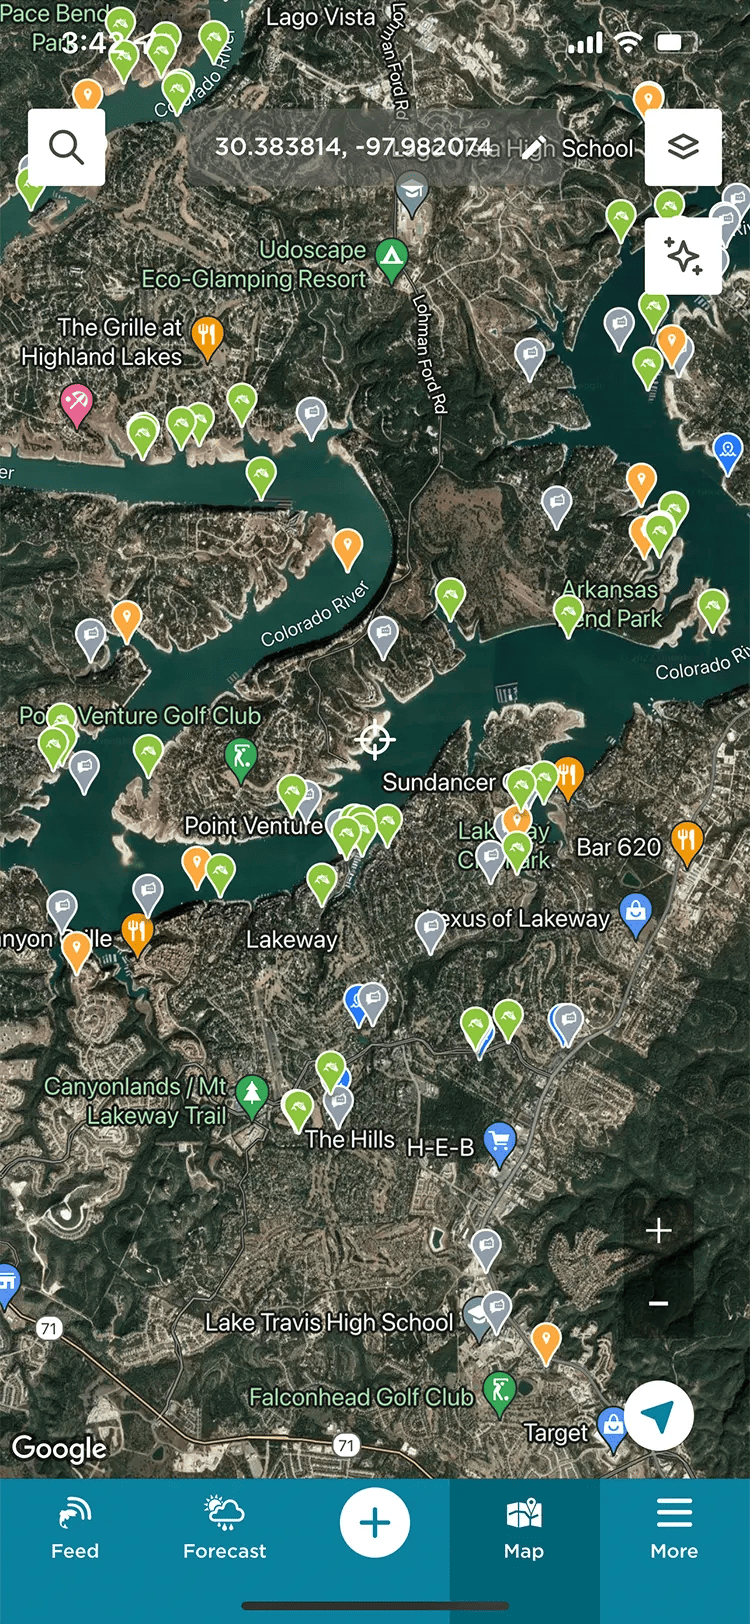
\includegraphics[scale=0.25]{./dados/figuras/fish-angler-app-map}
    \fonte{\citeonline{FishAngler24}}
\end{figure}

Apesar deste aplicativo possuir muitas funcionalidades e recursos, este não conta com a tradução para o português,o que resulta em uma baixa adesão por parte dos brasileiros, em sua maioria, não familiarizados com a língua inglesa.

Outro produto que possui funcionalidades semelhantes ao esperado para este projeto é a ferramenta \textit{FishFriender}, que conta com um aplicativo móvel e também uma página \textit{Web}. O aplicativo dispõe de funcionalidades como registrar peixes, registrar sessões de pesca e a possibilidade de compartilhar as informações com outros usuários.

A principal página do aplicativo móvel está sendo apresentada na Figura \ref{fig:fishFrienderApp}, esta conta com as principais capturas, os melhores contribuidores, propagandas, avisos e entre outras informações relacionadas às capturadas compartilhadas pelos usuários.

\begin{figure}[H]
    \centering
    \caption{FishFriender - Diario de pesca}
    \label{fig:fishFrienderApp}
    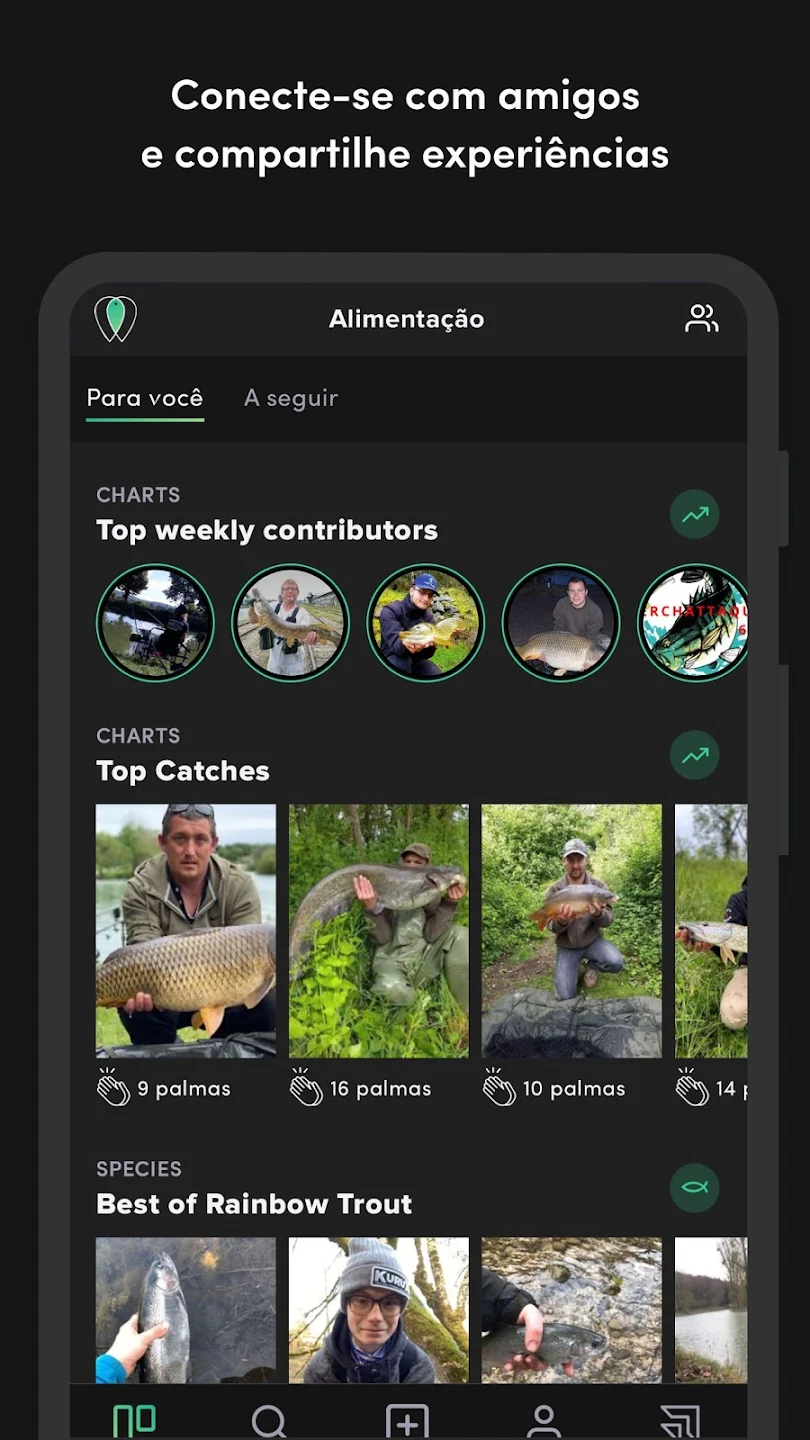
\includegraphics[scale=0.25]{./dados/figuras/fish-friender-app-feed}
    \fonte{\citeonline{FishFrienderPlayStore24}}
\end{figure}

Embora o aplicativo móvel ofereça diversas funcionalidades e recursos, ele não possui completa tradução para o português, o que acarreta ao semelhante problema do produto já citado neste documento.

\section{FERRAMENTAS E TECNOLOGIAS}
\label{sec:feramentasETecnologias}

As ferramentas, tecnologias e ambientes de desenvolvimento que serão utilizados no processo de desenvolvimento deste projeto são de \textit{open source} (código-fonte) ou possuem sua versão para a comunidade onde não é permitido o uso comercial ou empresarial. Segundo \citeonline{ferreira2005open} tecnologias open source são aquelas onde todos podem ter livre acesso para qualquer fim.

Para a criação da \textit{Application programming interface} (API) foi escolhido a plataforma de desenvolvimento .NET, esta conta com a linguagem de programação C\#, além de possuir diversas funcionalidades e recursos que facilitam o desenvolvimento de aplicativos, jogos, e entre outras ferramentas, como tratado pela documentação oficial da \citeonline{Microsoft24}.

O conjunto de bibliotecas Flutter foi escolhido para criar a aplicação móvel, a página web oficial do \citeonline{FlutterWeb24} descreve que o \textit{framework} utiliza a linguagem de programação multiplataforma Dart, e tem como premissa atender usuários de diversas plataformas com apenas um código-fonte.

Visual Studio e Visual Studio Code serão os ambientes de desenvolvimento  utilizados durante o processo de desenvolvimento. O Visual Studio Code conta com sua versão de código aberto, livre de restrições comerciais ou monetárias; o Visual Studio possui sua versão comunitária onde o uso é restrito para fins educacionais.

\section{PERSISTÊNCIA DE DADOS}
\label{sec:persistenciaDeDados}

Para a persistência dos dados será utilizado o banco de dados não relacional orientado a documentos MongoDB, escolha feita devido à sua alta flexibilidade com gerenciamento de dados. O MongoDB conta com seu armazenamento utilizando objetos \textit{JavaScript Object Notation} (JSON), tornando mais fácil incluir novas propriedades, criar novas relações, entre outras possibilidades. 

Segundo a página do \citeonline{MongoDB24}, a plataforma conta com diversos recursos que podem auxiliar o desenvolvedor a gerenciar e estruturar os dados com mais agilidade. O MongoDB Compass ambiente utilizado para gerenciar conexões e dados, é um dos recursos proporcionados pela plataforma e será utilizado durante o desenvolvimento do projeto.

                      % Referencial teorico
% DESENVOLVIMENTO--------------------------------------------------------

\chapter{DESENVOLVIMENTO}
\label{chap:desenvolvimento}

\section{DIAGRAMA CASO DE USO}
\label{sec:diagramacasodeuso}

Neste tópico, será apresentado o diagrama de caso de uso, o qual é responsável por mostrar quais as funcionalidades de um sistema, e também quais os usuários com os quais interagem. De forma simples, é semelhante a um mapa que descreve os objetivos dos usuários ao usar o sistema.

\begin{figure}[H]
    \centering
    \caption{Diagrama de Caso de Uso}
    \label{fig:casoDeUso}
    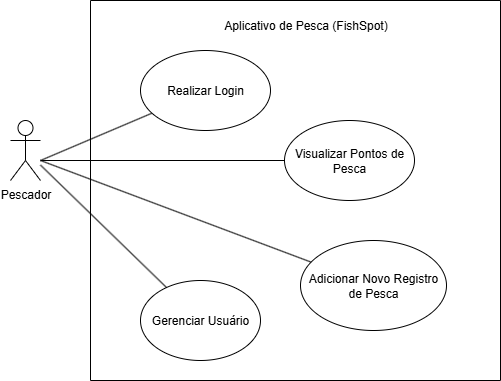
\includegraphics[scale=0.8]{./dados/figuras/diagrama-de-caso-de-uso.png}
    \fonte{\citeonline{DrawIO}}
\end{figure}


\section{DIAGRAMA DE CLASSE}
\label{sec:diagramadeclasse}

O diagrama de classe constitui uma ferramenta muito utilizada para a modelagem estática e estrutural de um sistema. A representação das classes, dos atributos, dos métodos e também suas relações, de forma visual, facilita a compreensão da arquitetura lógica do software.

\begin{figure}[H]
    \centering
    \caption{Diagrama de Classe}
    \label{fig:casoDeUso}
    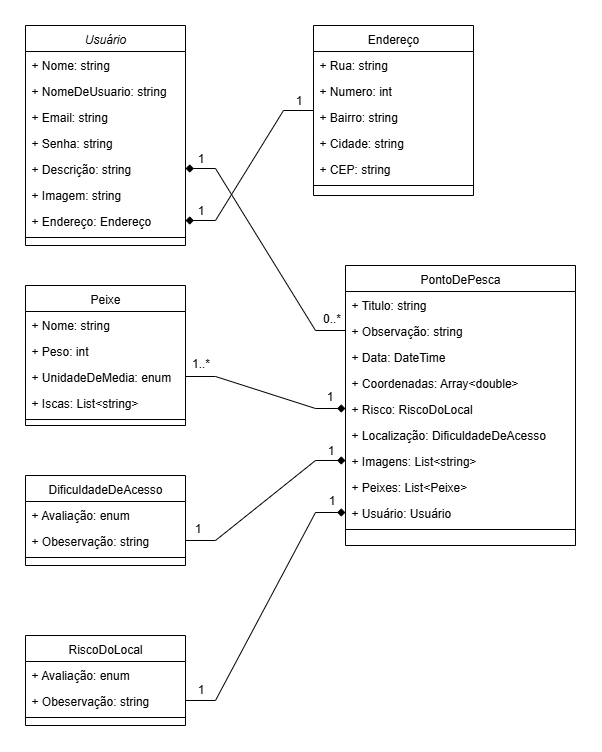
\includegraphics[scale=0.70]{./dados/figuras/diagrama-de-classe.png}
    \fonte{\citeonline{DrawIO}}
\end{figure}

\section{LEVANTAMENTO DE REQUISITOS}\label{sec:levantamentoderequisitos}

De acordo com \citeonline{fernandoCunha2025}, os requisitos funcionais são aqueles que representam funcionalidades às quais estão relacionados a ações dentro da solução proposta. Enquanto os funcionais estão relacionados a ações, os requisitos não funcionais estão relacionados a descrever a forma como serão feitos.

A \autoref{tab:tb-rf-realizar-login} aborda os requisitos para a realização do login, onde o pescador informa as credenciais de acesso, e recebe permissões para navegação dentro da aplicação. Além disso, são descritos seus requisitos não funcionais atrelados.

\begin{table}[h!]
    \centering
    \caption[Requisitos de Autenticação do Usuário]{Requisitos de Autenticação do Usuário
    \label{tab:tb-rf-realizar-login}}
    \setlength{\extrarowheight}{2pt}
    \begin{tabular}{|l!{\vrule width 1pt}p{0.55\textwidth}|c|c|}
        \hline
        \textbf{RF-1} & \multicolumn{3}{|l|}{Realizar Login} \\
        \hline
        \multicolumn{4}{|p{0.9\textwidth}|}{\textbf{Descrição detalhada:} } \\
        \hline
        \multicolumn{4}{|c|}{\textbf{REQUISITOS NÃO FUNCIONAIS ASSOCIADOS}} \\
        \hline
        \textbf{Nome} & \textbf{Restrição} & \textbf{Categoria} & \textbf{Desejável} \\
        \hline
        RNF1.1 & Os dados sensíveis do usuário devem ser criptografados durante o processo de autenticação & Segurança & Obrigatório \\
        \hline
        RNF1.2 & A duração do processo de autenticação não deve ser longo  & Desempenho & Obrigatório \\
        \hline
        RNF1.3 & O usuário não deve conseguir acessar o aplicativo sem ser autenticado & Usabilidade & Obrigatório \\
        \hline
        RNF1.4 & A interface deve seguir os padrões gerais de design para deixar mais intuitiva e acessível & Usabilidade & Obrigatório \\
        \hline
    \end{tabular}
    \fonte{Fonte: Produzido pelo Autor}
\end{table}

A \autoref{tab:tb-rf-visualizar-pontos-pesca} descreve os requisitos para visualizar um ponto de pesca, onde o usuário visualiza todos os pontos de pesca cadastrados, bem como seus detalhes. São detalhados também os requisitos não funcionais relacionados, dentre eles visualização do mapa, cálculos de geolocalização, localização atual do usuário e etc.

\begin{table}[h!]
    \centering
    \caption[Requisitos para Visualização Pontos de Pesca]{Requisitos para Visualização de Pontos de Pesca
    \label{tab:tb-rf-visualizar-pontos-pesca}}
    \setlength{\extrarowheight}{2pt}
    \begin{tabular}{|l!{\vrule width 1pt}p{0.55\textwidth}|c|c|}
        \hline
        \textbf{RF-2} & \multicolumn{3}{|l|}{Visualizar Pontos de Pesca} \\
        \hline
        \multicolumn{4}{|p{0.9\textwidth}|}{\textbf{Descrição detalhada:} } \\
        \hline
        \multicolumn{4}{|c|}{\textbf{REQUISITOS NÃO FUNCIONAIS ASSOCIADOS}} \\
        \hline
        \textbf{Nome} & \textbf{Restrição} & \textbf{Categoria} & \textbf{Desejável} \\
        \hline
        RNF2.1 & Durante visualização dos pontos de pesca, dados sensíveis dos outros usuários não devem ser expostos & Segurança & Obrigatório \\
        \hline
        RNF2.2 & Os pontos de pesca devem ser exibidos em um mapa, semelhante às aplicações Waze, Google Maps e etc. & Usabilidade & Obrigatório \\
        \hline
        RNF2.3 & Deve ser possivel visualizar os pontos de pesca de forma singular, exibindo detalhes do registro feito & Usabilidade & Obrigatório \\
        \hline
        RNF2.4 & Deve ser possivel visualizar as fotos registradas nos detalhes do ponto de pesca  & Usabilidade & Desejável \\
        \hline
        RNF2.5 & As informações devem ser exibidas de forma fluidas e o mapa não deve demorar para renderizar os pontos de pesca & Desempenho & Obrigatório \\
        \hline
    \end{tabular}
    \fonte{Fonte: Produzido pelo Autor}
\end{table}

Os requisitos relacionados ao cadastro de um novo ponto de pesca é representado pela \autoref{tab:tb-rf-novo-registro-pesca}, onde detalha as principais características da funcionalidade, também como seus requisitos não funcionais.

\begin{table}[h!]
    \centering
    \caption[Requisitos de Cadastro de Pontos de Pesca]{Requisitos de Cadastro de Pontos de Pesca
    \label{tab:tb-rf-novo-registro-pesca}}
    \setlength{\extrarowheight}{2pt}
    \begin{tabular}{|l!{\vrule width 1pt}p{0.55\textwidth}|c|c|}
        \hline
        \textbf{RF-3} & \multicolumn{3}{|l|}{Adicionar Novo Registro de Pesca} \\
        \hline
        \multicolumn{4}{|p{0.9\textwidth}|}{\textbf{Descrição detalhada:} } \\
        \hline
        \multicolumn{4}{|c|}{\textbf{REQUISITOS NÃO FUNCIONAIS ASSOCIADOS}} \\
        \hline
        \textbf{Nome} & \textbf{Restrição} & \textbf{Categoria} & \textbf{Desejável} \\
        \hline
        RNF3.1 & Deve ser possível incluir fotos dos peixes capturados durante a pesca & Usabilidade & Obrigatório  \\
        \hline
        RNF3.2 & As iscas utilizadas durante o processo devem ser incluídas & Usabilidade & Obrigatório \\
        \hline
        RNF3.3 & Informações sobre o percurso e sobre riscos devem ser informadas & Usabilidade & Desejavel \\
        \hline
        RNF3.4 & A aplicação deve ser rápida para persistir os dados informados & Desempenho & Obrigatório \\
        \hline
        RNF3.5 & Os dados devem ser armazenados corretamente, para que a confiabilidade das informações sejam mantidas & Segurança & Obrigatório  \\
        \hline
    \end{tabular}
    \fonte{Fonte: Produzido pelo Autor}
\end{table}

Na \autoref{tab:tb-rf-gerenciar-usuario}, os requisitos para gerenciar o usuário são descritos. Nesta funcionalidade é feito o gerenciamento dos dados do usuário, o gerenciamento esta atrelado a incluir, editar e também visualizar os dados dos pescadores.

\begin{table}[h!]
    \centering
    \caption[Requisitos de Gerenciamento do Usuário]{Requisitos de Gerenciamento do Usuário
    \label{tab:tb-rf-gerenciar-usuario}}
    \setlength{\extrarowheight}{2pt}
    \begin{tabular}{|l!{\vrule width 1pt}p{0.55\textwidth}|c|c|}
        \hline
        \textbf{RF-4} & \multicolumn{3}{|l|}{Gerenciar Usuário} \\
        \hline
        \multicolumn{4}{|p{0.9\textwidth}|}{\textbf{Descrição detalhada:} } \\
        \hline
        \multicolumn{4}{|c|}{\textbf{REQUISITOS NÃO FUNCIONAIS ASSOCIADOS}} \\
        \hline
        \textbf{Nome} & \textbf{Restrição} & \textbf{Categoria} & \textbf{Desejável} \\
        \hline
        RNF4.1 & O usuário deve conseguir visualizar seus pontos de pescas cadastrados & Usabilidade & Obrigatório \\
        \hline
        RNF4.2 & O usuário terá a possibilidade de excluir os pontos de pescas cadastrados & Usabilidade & Obrigatório  \\
        \hline
        RNF4.3 & O usuário deve ser capaz de alterar os dados relacionados ao cadastro & Usabilidade & Obrigatório \\
        \hline
        RNF4.4 & O usuário deve conseguir cancelar a autenticação na aplicação e eventualmente encerrar o uso & Usabilidade & Obrigatório \\
        \hline
        RNF4.5 & Após o encerramento da autenticação, nenhum dado sensível deve ser mantido na aplicação & Segurança & Obrigatório \\
        \hline
    \end{tabular}
    \fonte{Fonte: Produzido pelo Autor}
\end{table}

A \autoref{tab:tb-rnf-autonomos} descreve os requisitos não-funcionais autônomos, estes que não são totalmente relacionados a uma funcionalidade e sim focados a outros aspectos da aplicação.

\begin{table}[h!]
    \centering
    \caption[Requisitos de Visualização de Pontos de Pesca]{Requisitos de Visualização de Pontos de Pesca
    \label{tab:tb-rnf-autonomos}}
    \setlength{\extrarowheight}{2pt}
    \begin{tabular}{|l!{\vrule width 1pt}p{0.55\textwidth}|c|c|} 
        \hline
        \multicolumn{4}{|c|}{\textbf{REQUISITOS NÃO FUNCIONAIS AUTÔNOMOS}} \\
        \hline
        \textbf{Nome} & \textbf{Restrição} & \textbf{Categoria} & \textbf{Desejável} \\
        \hline
         RNF-A.1 & A interface gráfica da aplicação móvel deve ser desenvolvida em Flutter & Padrão & Obrigatório  \\
        \hline
         RNF-A.2 & O Bando de Dados do sistema deve ser MongoDB & Padrão & Obrigatório  \\
        \hline
         RNF-A.3 & A API deve ser desenvolvida utilizando .NET & Padrão & Obrigatório \\
        \hline
    \end{tabular}
    \fonte{Fonte: Produzido pelo Autor}
\end{table}

\section{DIAGRAMA DE ARQUITETURA DE SOFTWARE}
\label{sec:diagramadearquiteturadesoftware}

De acordo com a empresa \citeonline{AwsAmazon2024}, os diagramas de arquitetura fornecem vários benefícios; dentre eles, estão a redução de risco, eficiência e escalabilidade. Os diagramas ajudam a identificar os possíveis riscos no desenvolvimento, fornecendo uma visualização clara dos componentes e estruturas do sistema, possibilitando identificar também maneiras fáceis e eficientes de escalar o sistema. A \autoref{fig:diagramaArquiteturaDeSoftware} representa a arquitetura utilizada para criação do FishSpot.

\begin{figure}[H]
    \centering
    \caption{Diagrama de Arquitetura}
    \label{fig:diagramaArquiteturaDeSoftware}
    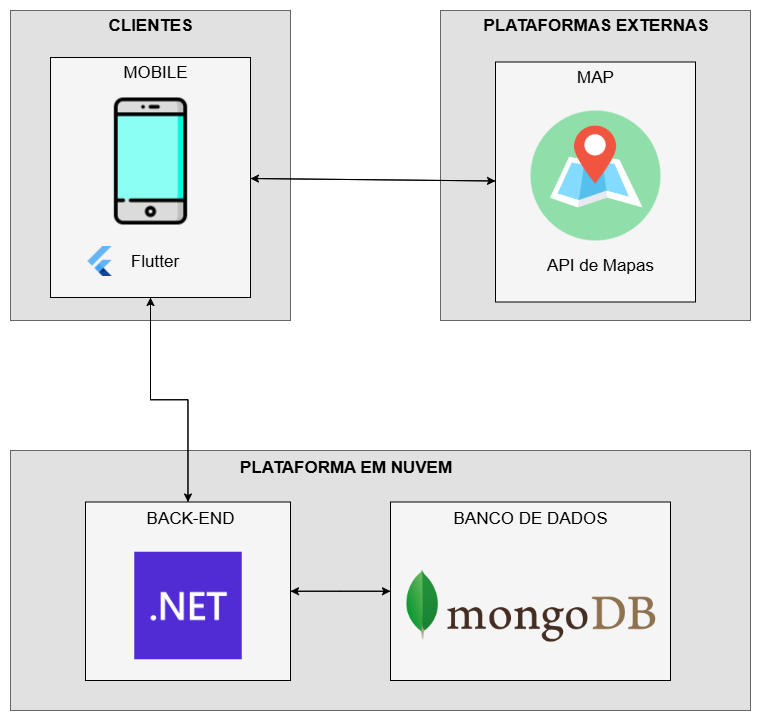
\includegraphics[scale=0.38]{./dados/figuras/diagrama-de-arquitetura.png}
    \fonte{\citeonline{DrawIO}}
\end{figure}

\section{PROTOTIPAGEM}
\label{sec:prototipagem}

Neste tópico vamos abordar a prototipagem, um processo extremamente necessário durante o desenvolvimento de um sistema. Segundo \citeonline{de2006prototipagem} a prototipagem tem a característica-chave de apresentar uma forma muito fácil de construir uma entidade temporária para que o produto possa ser visto é criticado, para então gerar novas melhorias.

É possível visualizar na \autoref{fig:prototipagemAutenticacaoUsuario} parte da prototipagem das telas relacionadas à autenticação de usuários, dentre elas estão: autenticação de usuário, registro de usuário e recuperação de senha.

\begin{figure}[H]
    \centering
    \caption{Prototipagem das Telas Relacionadas a Autenticação}
    \label{fig:prototipagemAutenticacaoUsuario}
    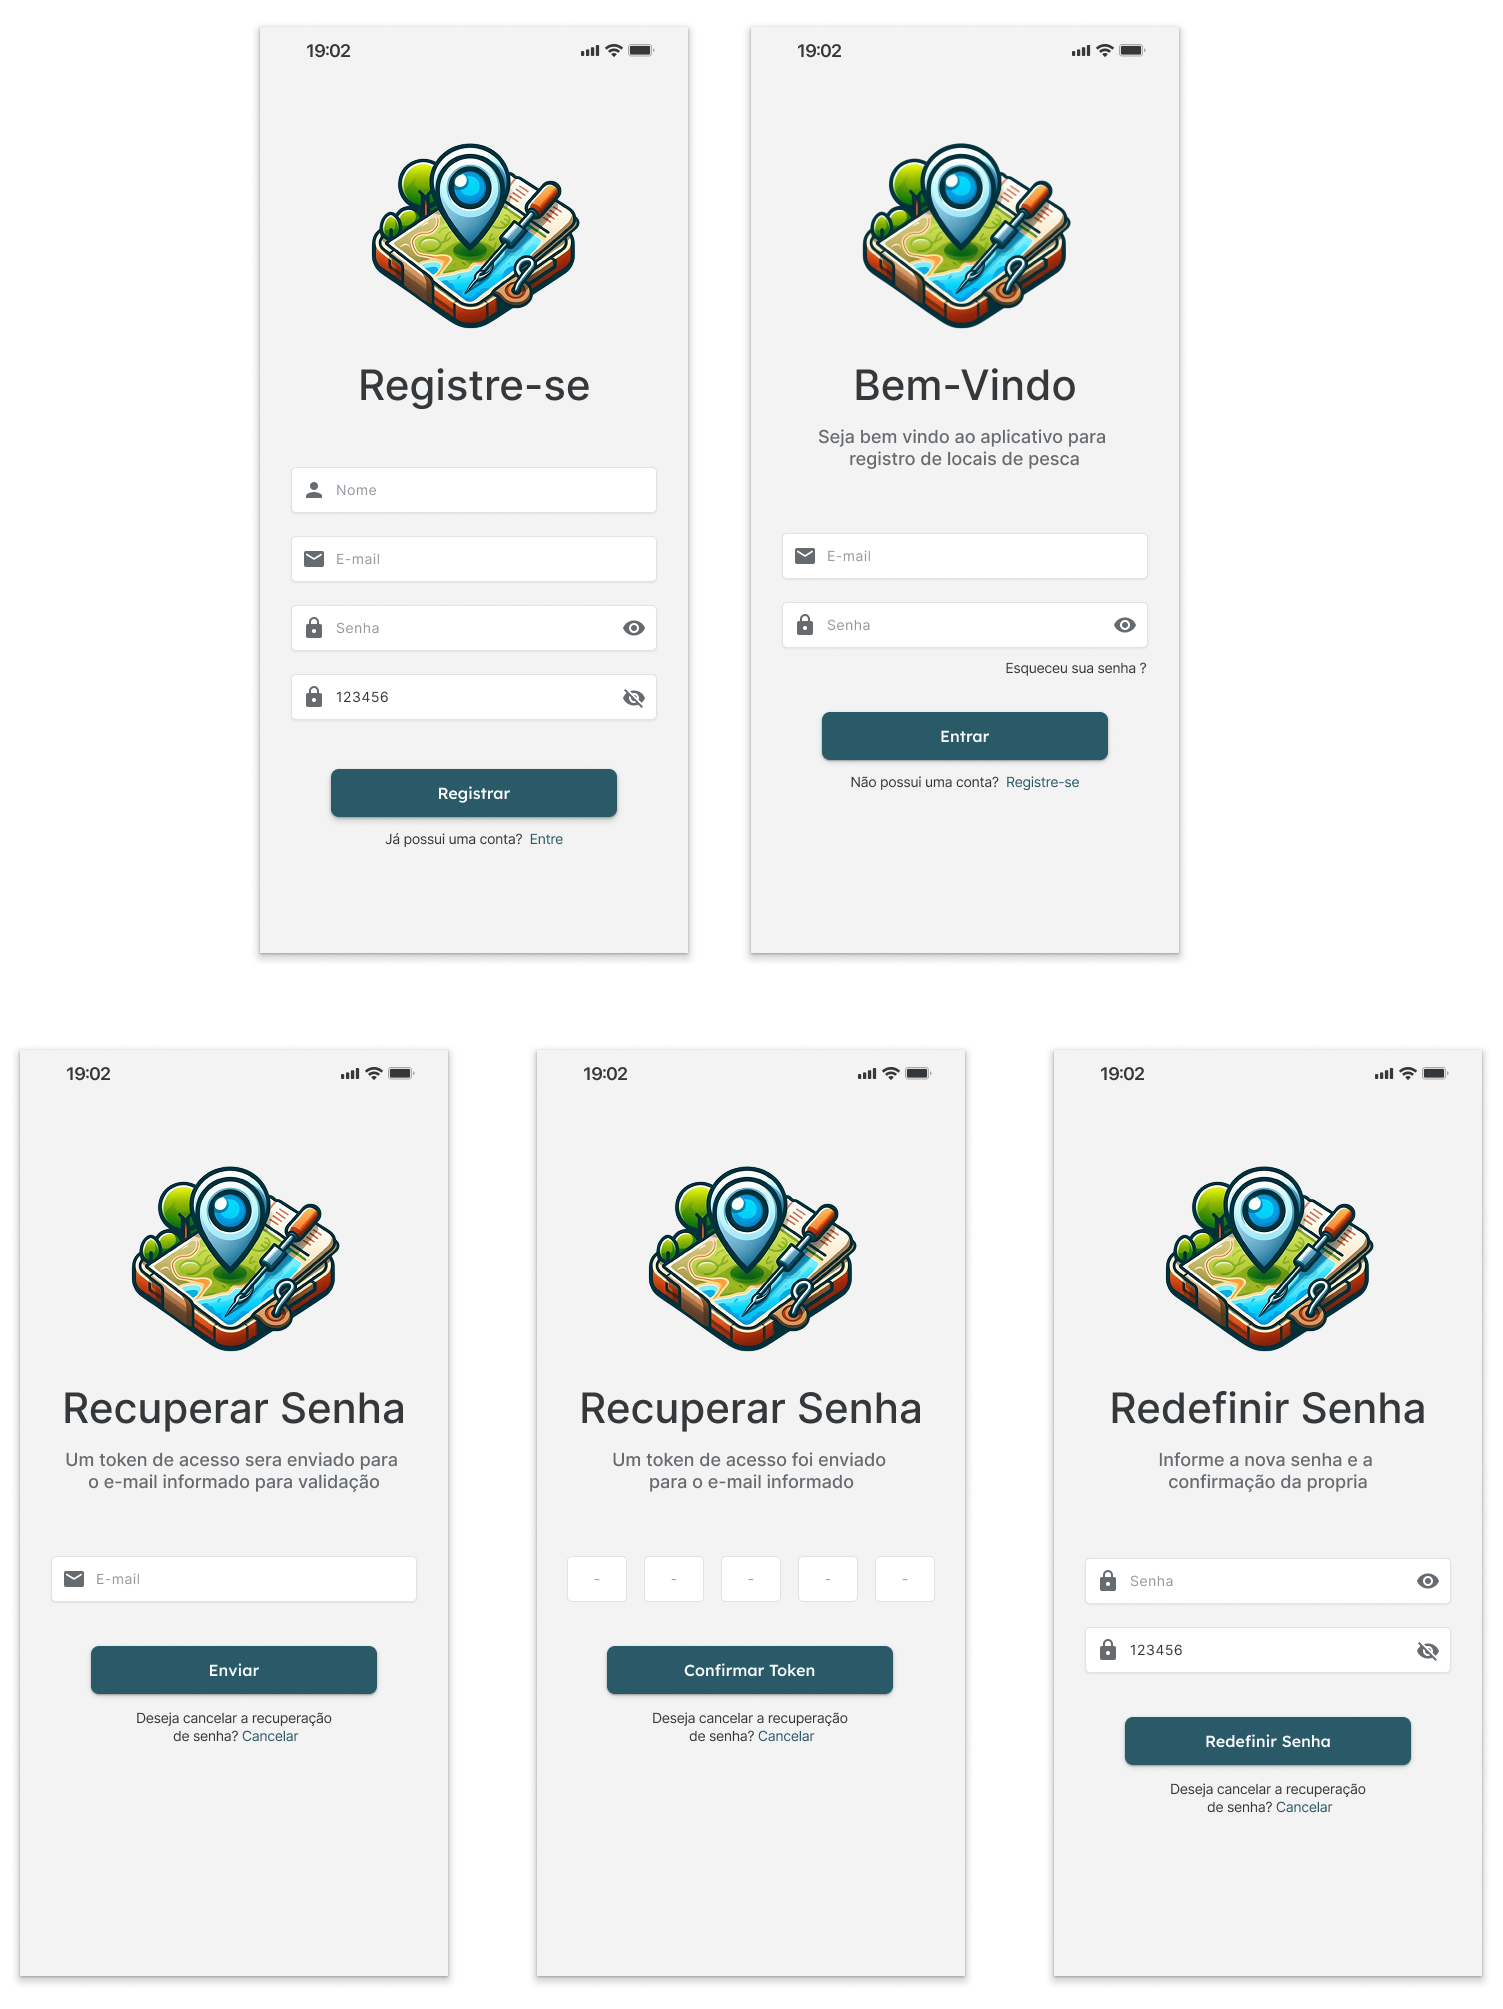
\includegraphics[scale=0.24]{./dados/figuras/prototipagem-autenticacao-de-usuario.png}
    \fonte{Produzido pelo Autor}
\end{figure}

A \autoref{fig:prototipagemMapPerfil} representa a prototipagem das telas relacionadas aos recursos de mapa e perfil do usuário, dentre elas estão o mapa, a visualização do ponto de pesca, perfil do pescador(a), edição do perfil do pescador(a) e uma futura tela de configuração.

\begin{figure}[H]
    \centering
    \caption{Prototipagem do Mapa e Perfil do Usuário}
    \label{fig:prototipagemMapPerfil}
    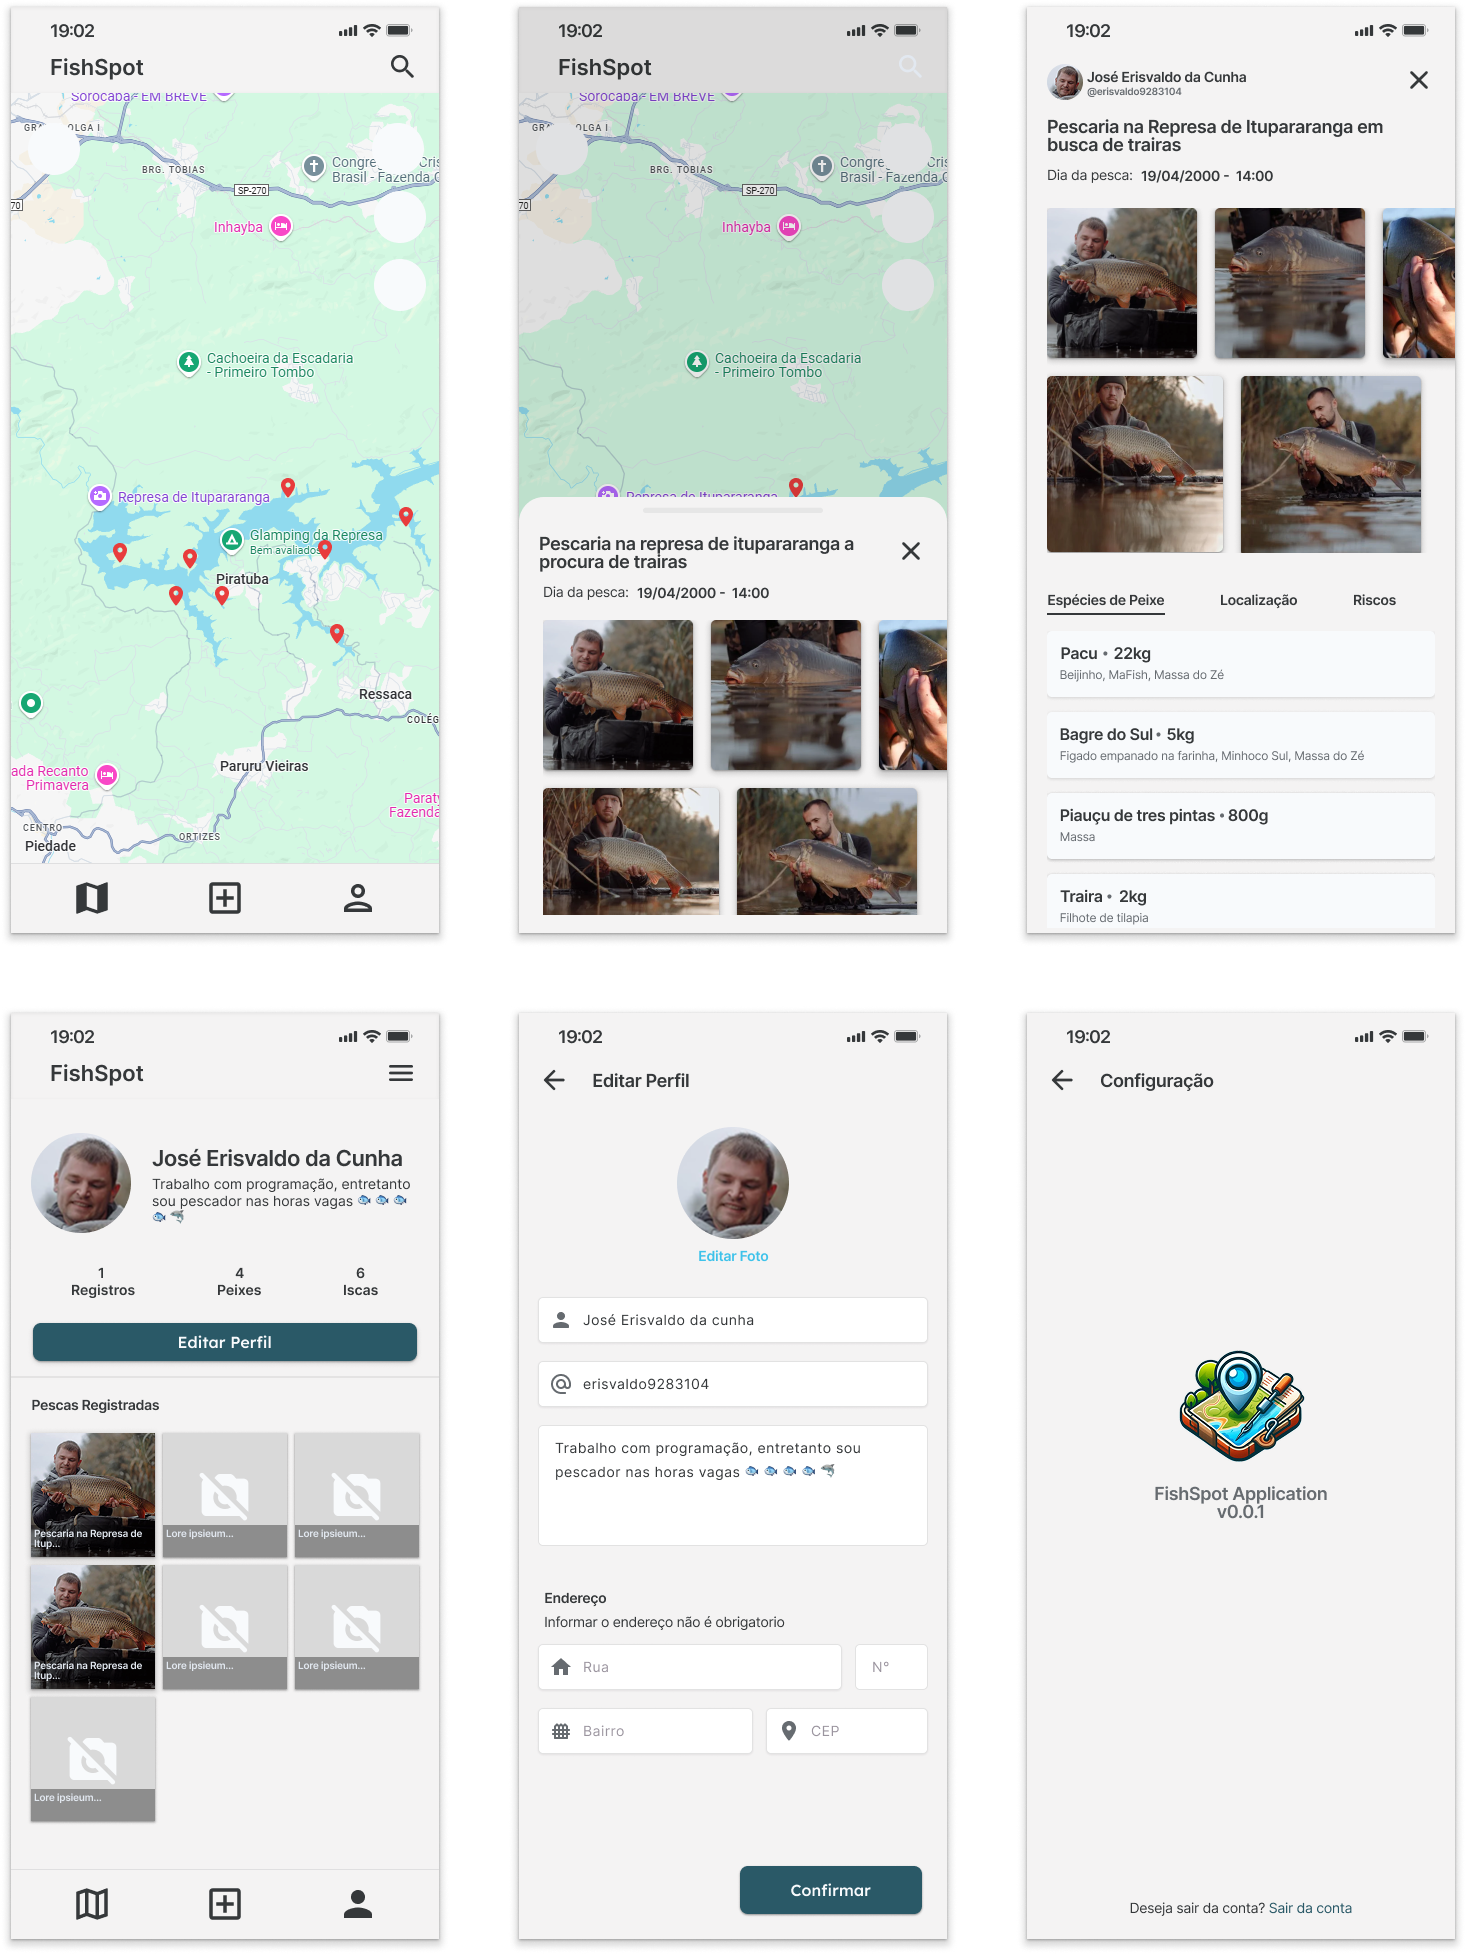
\includegraphics[scale=0.29]{./dados/figuras/prototipagem-map-perfil.png}
    \fonte{Produzido pelo Autor}
\end{figure}

A \autoref{fig:prototipagemRegisterSpot} apresenta a prototipagem das telas relacionadas ao registro dos pontos de pesca, dentre elas estão: descrição de riscos, inclusão de imagem, inclusão das iscas usadas e peixes pegos, inclusão de dados finais sobre o ponto.

\begin{figure}[H]
    \centering
    \caption{Prototipagem do Registro do Ponto de Pesca}
    \label{fig:prototipagemRegisterSpot}
    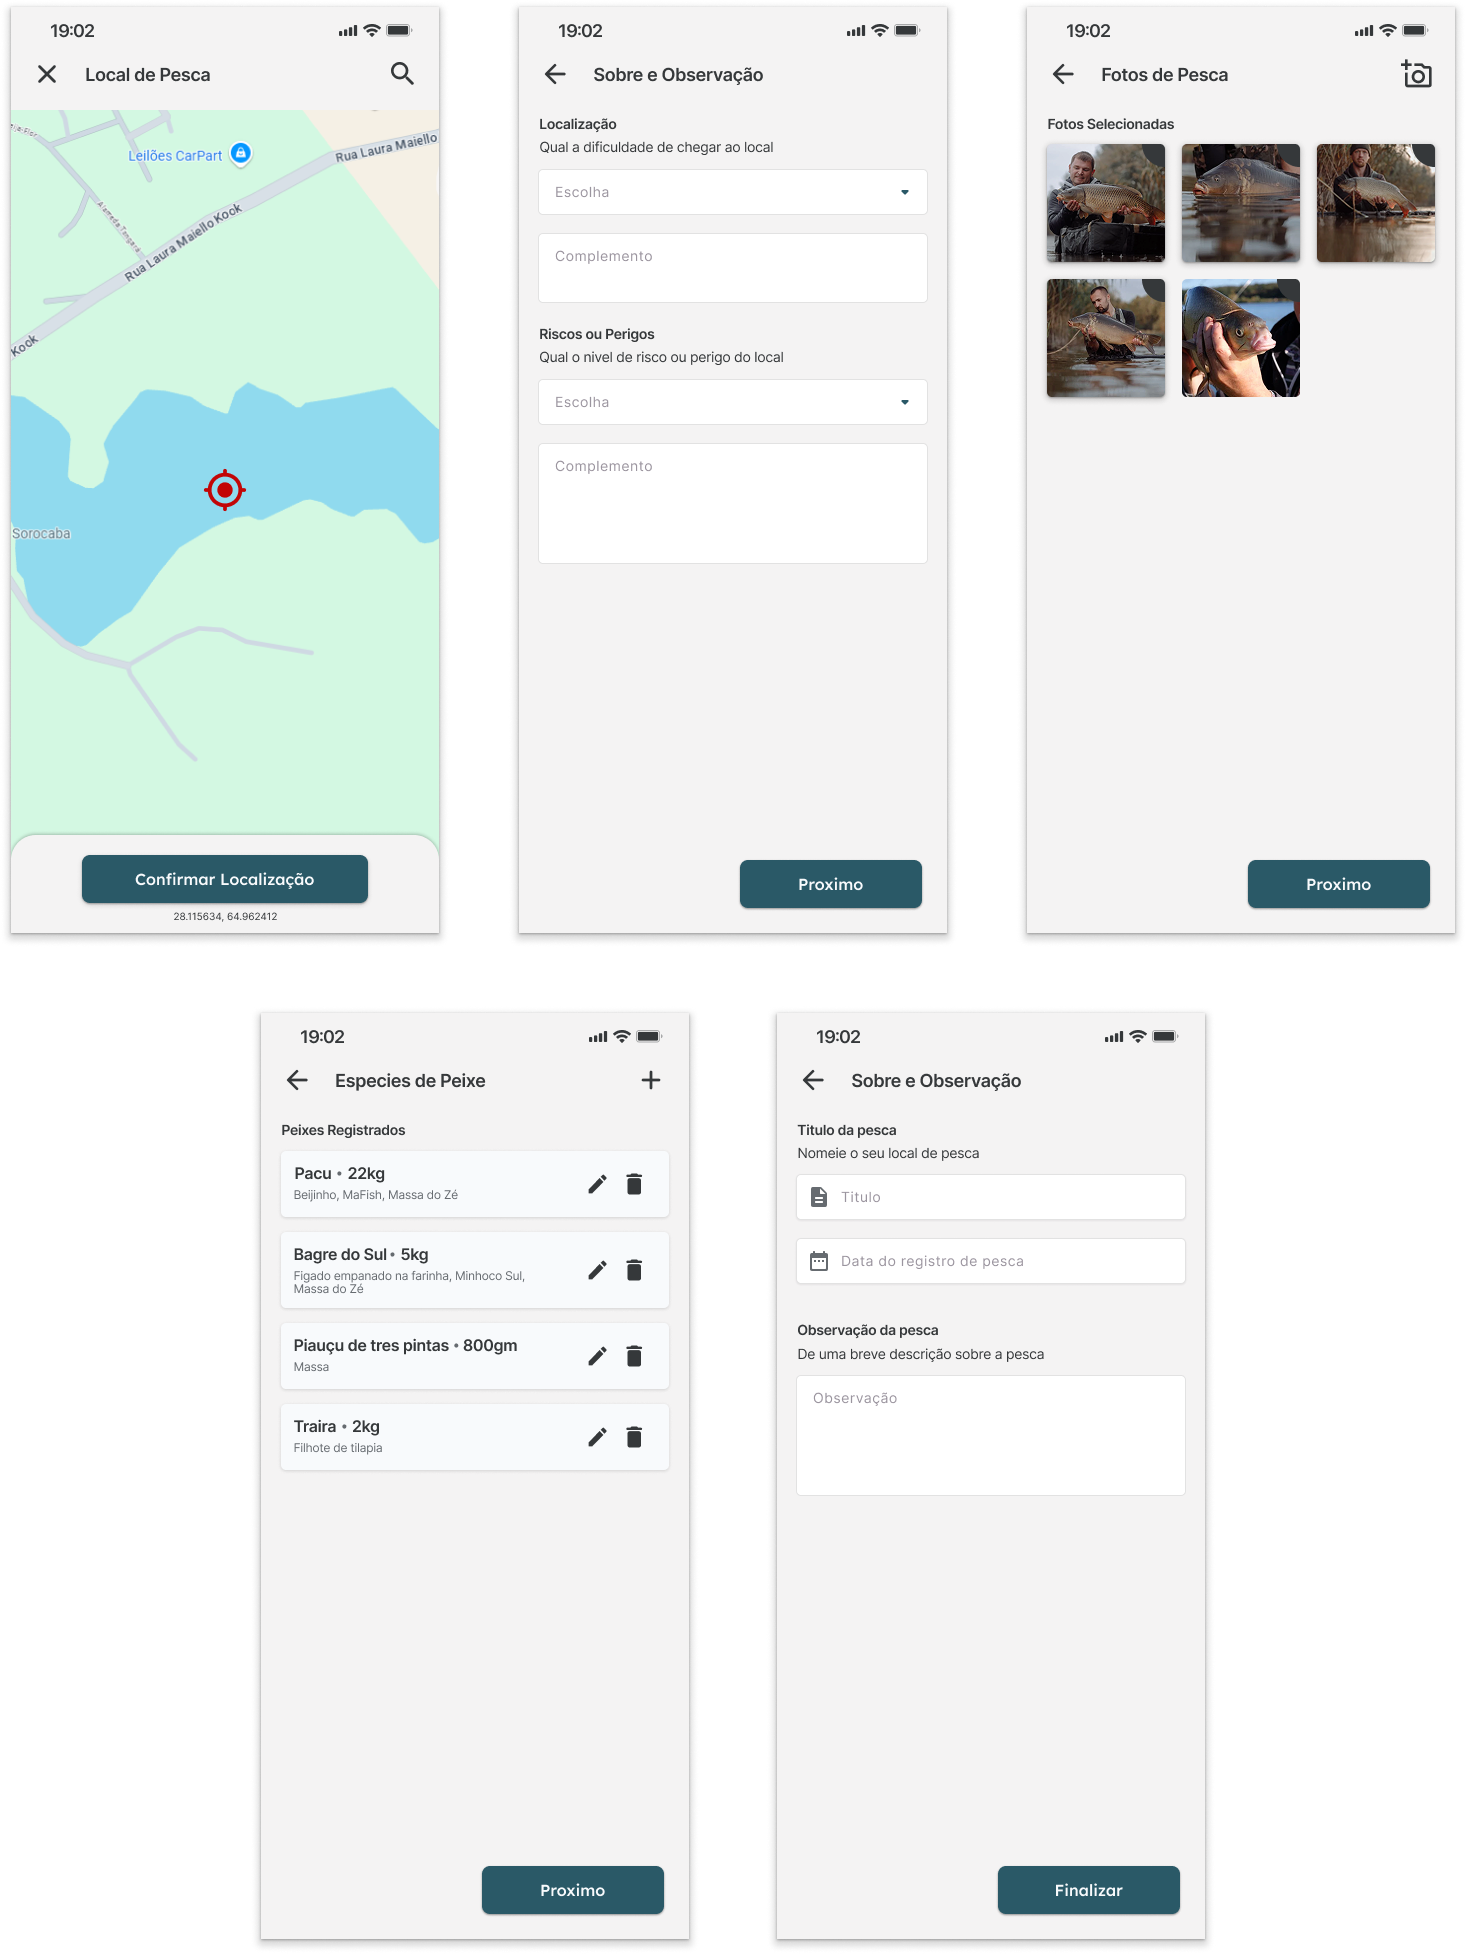
\includegraphics[scale=0.29]{./dados/figuras/prototipagem-spot-register.png}
    \fonte{Produzido pelo Autor}
\end{figure}


Pode-se observar na \autoref{fig:prototipagemAutenticacaoUsuarioDark} a prototipagem das telas de autenticação do usuário, destacando o modo escuro. Este que aumenta  usabilidade e cria maior conforto visual, reduzindo a fadiga ocular.

\begin{figure}[H]
    \centering
    \caption{Prototipagem das Telas Relacionadas a Autenticação no Modo Escuro}
    \label{fig:prototipagemAutenticacaoUsuarioDark}
    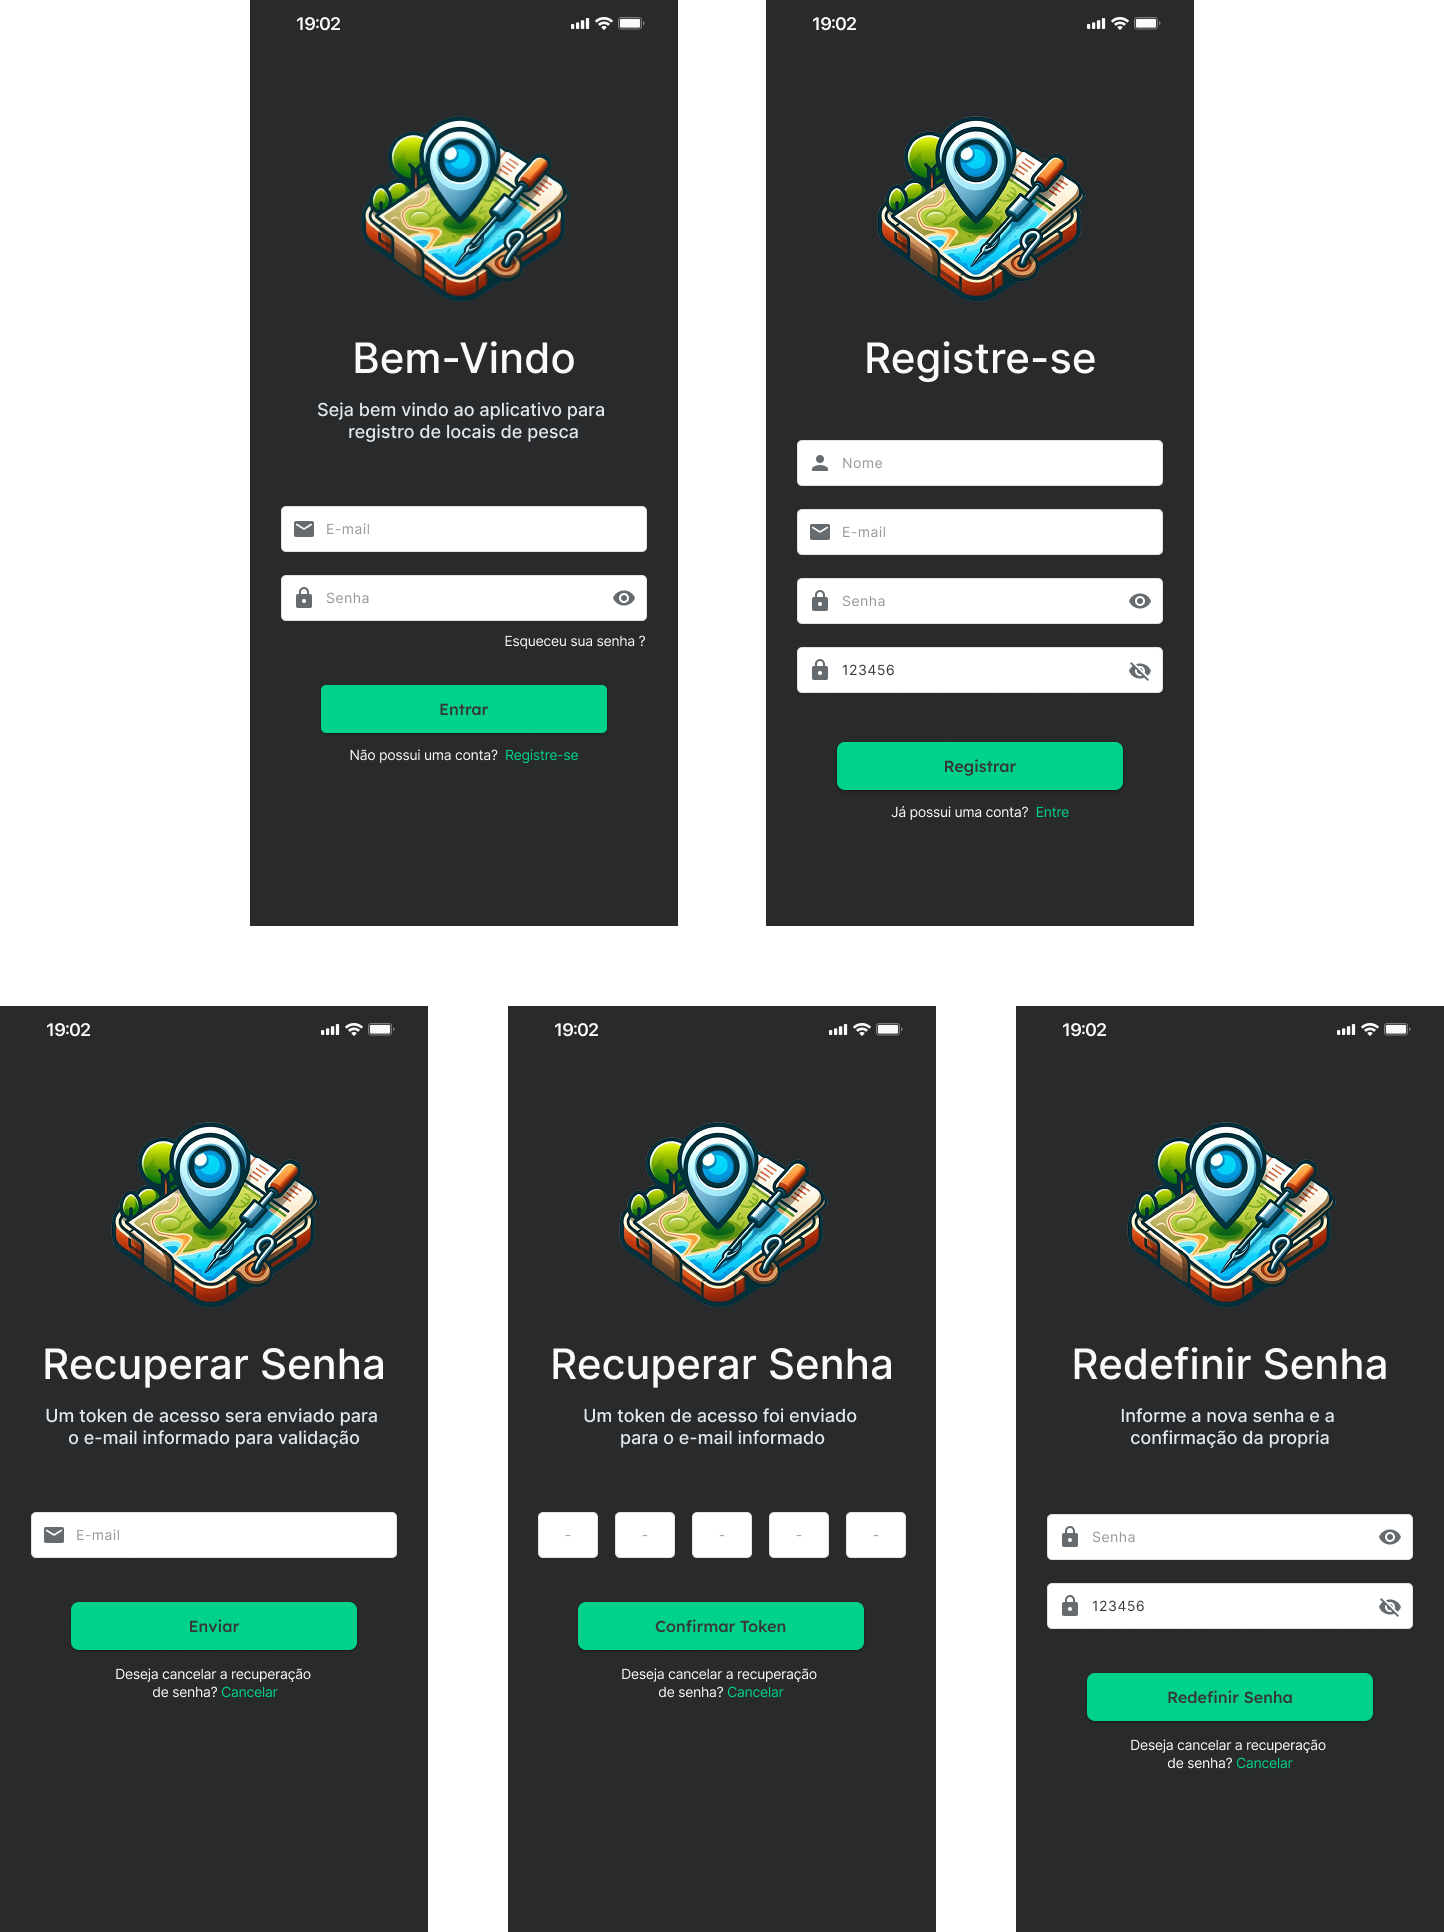
\includegraphics[scale=0.30]{./dados/figuras/prototipagem-dark-autenticacao-user.png}
    \fonte{Produzido pelo Autor}
\end{figure}

A \autoref{fig:prototipagemMapPerfilDark} exibe a prototipagem das telas de visualização dos pontos de pesca registrados, destacando o modo escuro da interface. Este que pode aumentar de forma significativa a economia no consumo de bateria do dispositivo móvel.

\begin{figure}[H]
    \centering
    \caption{Prototipagem do Mapa e Perfil do Usuário no Modo Escuro}
    \label{fig:prototipagemMapPerfilDark}
    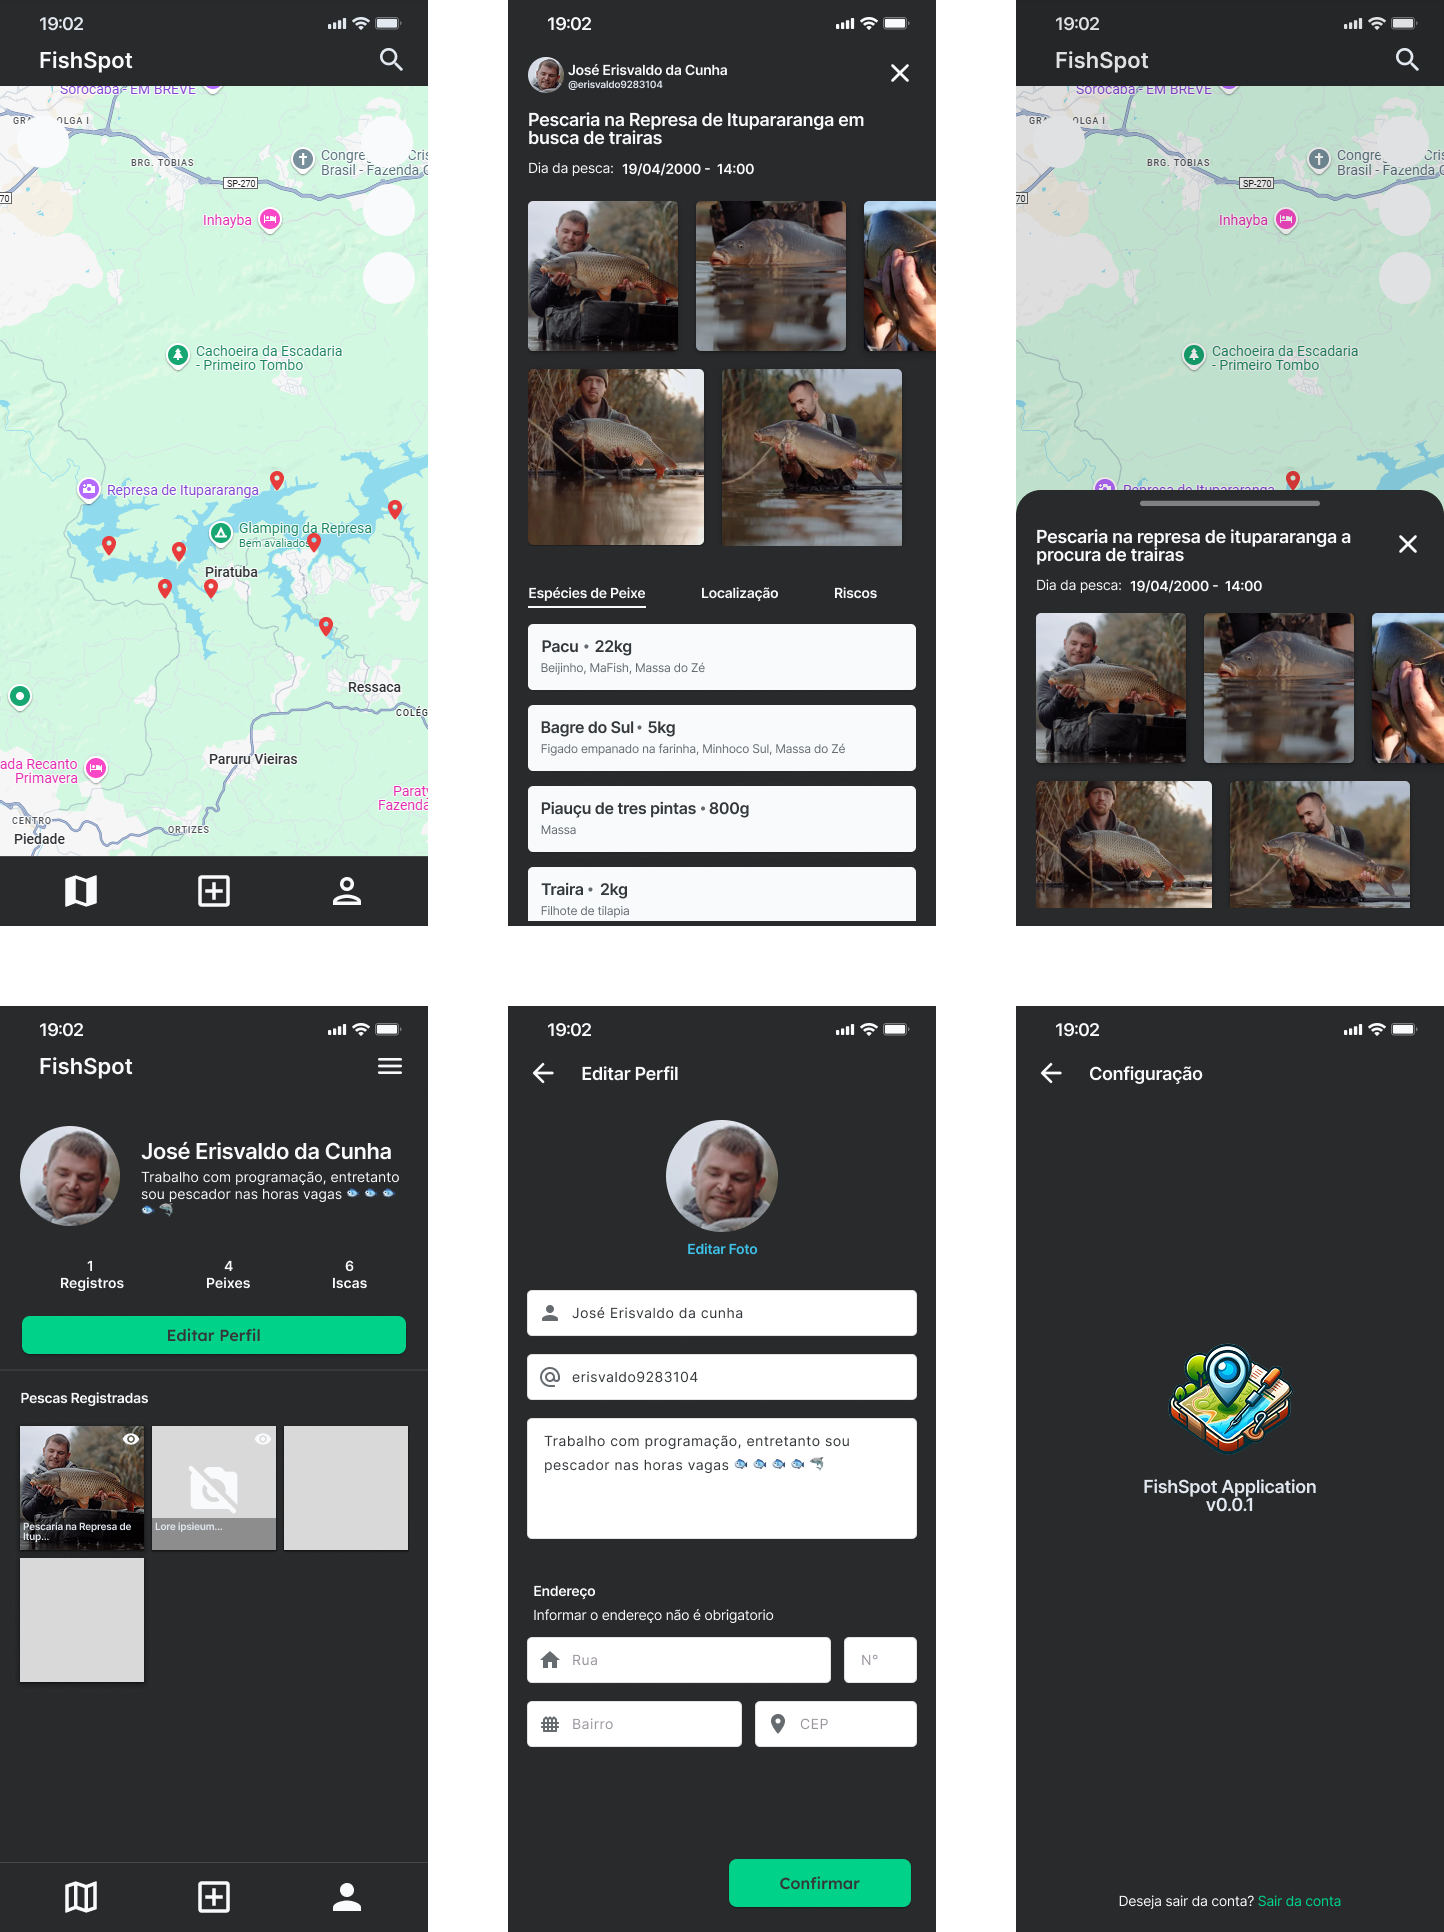
\includegraphics[scale=0.30]{./dados/figuras/prototipagem-dark-map-perfil.png}
    \fonte{Produzido pelo Autor}
\end{figure}

A \autoref{fig:prototipagemSpotRegisterDark} demonstra a prototipagem das telas de registro de pontos de pesca, destacando o modo escuro da interface. Este que busca atender às preferencias individuais e às necessidades de acessibilidade de diferentes usuários.

\begin{figure}[H]
    \centering
    \caption{Prototipagem do Registro do Ponto de Pesca no Modo Escuro}
    \label{fig:prototipagemSpotRegisterDark}
    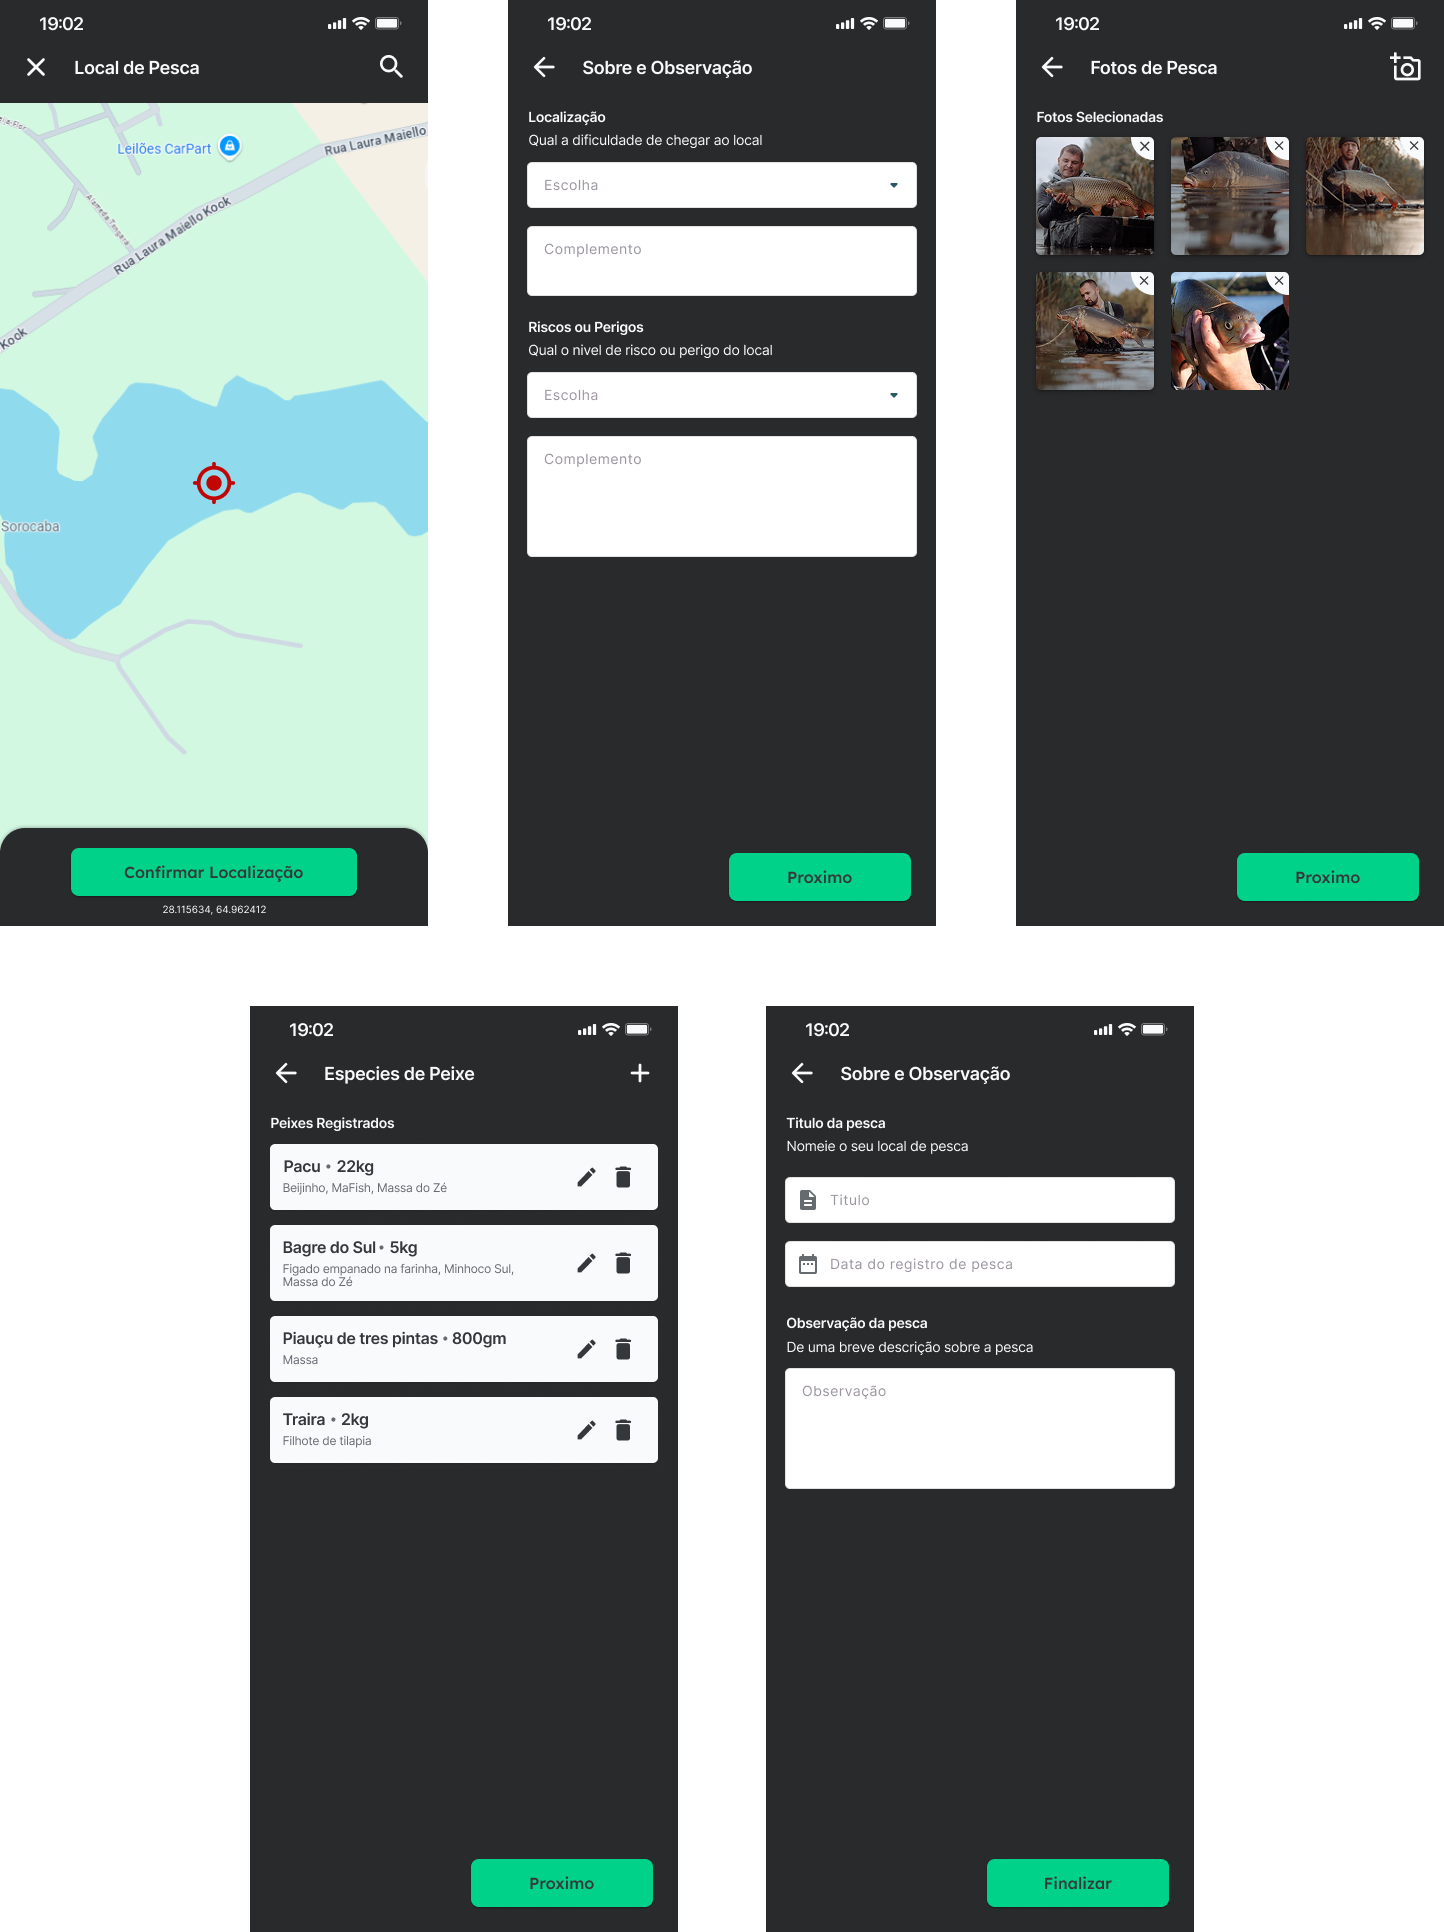
\includegraphics[scale=0.30]{./dados/figuras/prototipagem-dark-spot-register.png}
    \fonte{Produzido pelo Autor}
\end{figure}

\section{BANCO DE DADOS}
\label{sec:desenvolvimentobancodedados}

De acordo com a empresa \citeonline{MongoDBModelagem25}, detentora do banco de dados não relacional orientados a documento MongoDB. A criação de padroes de design de esquemas no banco de dados garantem de forma eficiente o armazenamento, a recuperação dos dados e a manipulação dos dados.

O diagrama ilustrado na \autoref{fig:documentacaoBancoDeDados}, representa a estrutura utilizado no banco de dados da aplicação, este que contem suas propriedades junto aos tipos utilizados, bem como sua relação.

\begin{figure}[H]
    \centering
    \caption{Documentação do Banco de Dados - MongoDB}
    \label{fig:documentacaoBancoDeDados}
    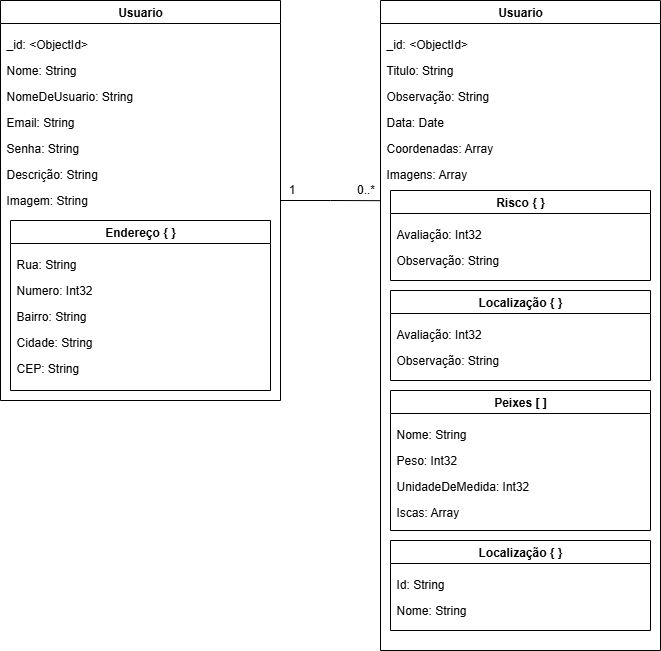
\includegraphics[scale=0.65]{./dados/figuras/documentacao-banco-de-dados.png}
    \fonte{Produzido pelo Autor}
\end{figure}                          % Desenvolvimento
% REFERENCIAL TEORICO---------------------------------------------------

\chapter{RESULTADO}
\label{chap:introducao}

Neste capitulo, serão detalhados os resultados obtidos nas telas da aplicação móvel, e também o resultado obtido no desenvolvimento da API. Na aplicação móvel, vão ser abordados assuntos como acessibilidade, usabilidade e a experiência do usuario. já na API, seram detalhadas as rotas criadas, bem como a documentação preparada.

\section{INTERFACE DE PROGRAMAÇÃO DE APLICAÇÕES}
\label{sec:resultadoApi}

Para documentar e descrever com clareza as rotas, a documentação Swagger foi utilizada. Segundo a documentação do \citeonline{SwaggerDoc2025}, tal produto visa criar uma documentação automática utilizando definições diretas da API, mantendo consistência e confiabilidade.. A \autoref{fig:docSwaggerAPI} exibe parte da documentação WEB gerada pela biblioteca Swagger istalada e configurada no projeto FishSpotAPI, nela é possivel realizar requisições HTTP, utilizar recursos de autenticação, e visualizar quais esquemas são usados nas requisições.

\begin{figure}[H]
    \centering
    \caption{Documentação Swagger - Rota de Autenticação}
    \label{fig:docSwaggerAPI}
    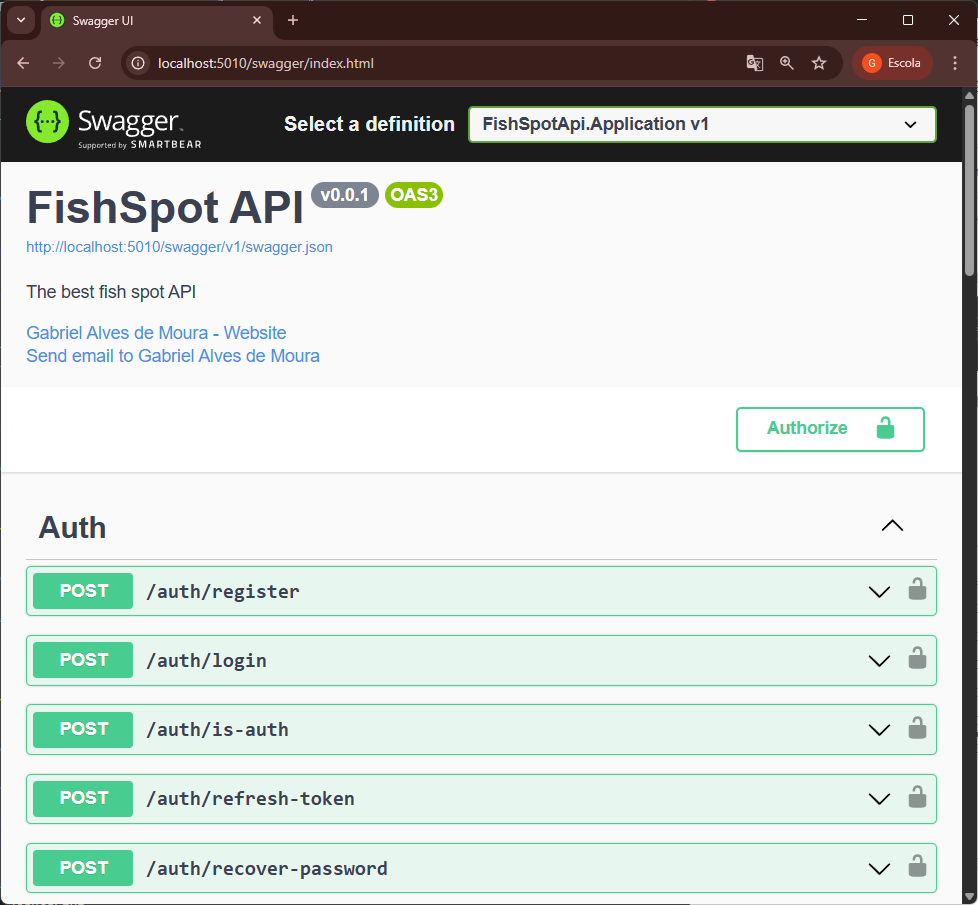
\includegraphics[scale=0.53]{./dados/figuras/api-swagger.png}
    \fonte{Produzido pelo Autor}
\end{figure}

A \autoref{fig:docSwaggerOthersAPI} exibe outra parte da documentação WEB gerada pela biblioteca Swagger istalada e configurada no projeto. Nesta parte exibida, podemos observar as rotas de recursos, de ponto de pesca e tambem de usuário.

\begin{figure}[H]
    \centering
    \caption{Documentação Swagger - Rota de Recursos, Ponto de Pesca e Usuário}
    \label{fig:docSwaggerOthersAPI}
    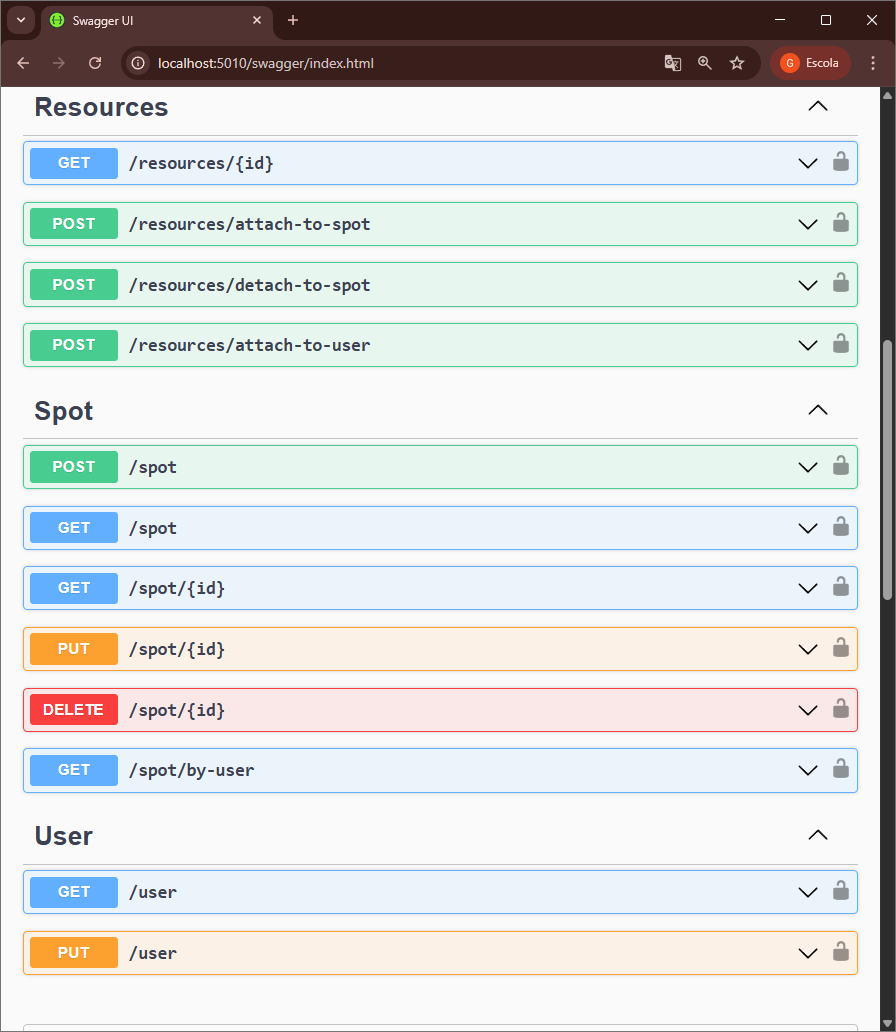
\includegraphics[scale=0.60]{./dados/figuras/swagger-api-others.png}
    \fonte{Produzido pelo Autor}
\end{figure}

\newpage

Pode-se observar na \autoref{fig:docSwaggerLoginAPI} o componente que pode ser usado para fazer uma requisição HTTP para a rota de Login. É possivel visualizar que é possivel incluir um corpo, parametros e visualizar qual o resultado obtido no final.

\begin{figure}[H]
    \centering
    \caption{Documentação Swagger - Documentação da Rota de Login}
    \label{fig:docSwaggerLoginAPI}
    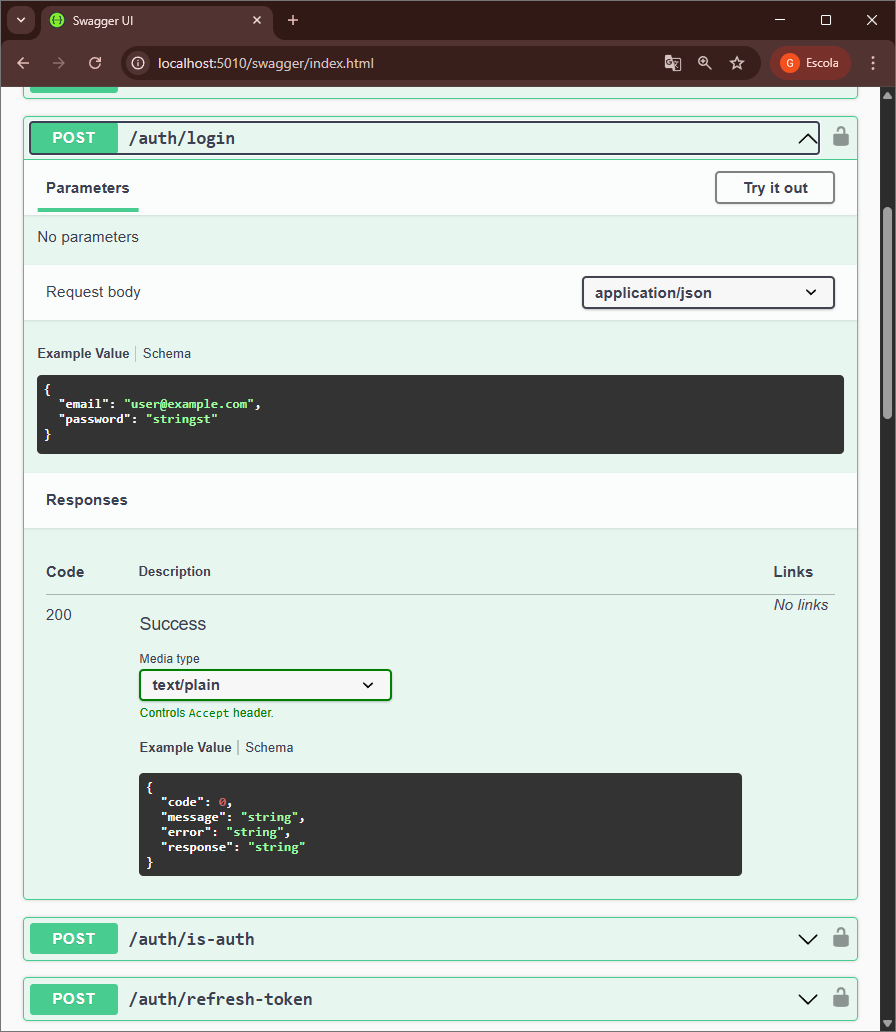
\includegraphics[scale=0.60]{./dados/figuras/swagger-api-login-doc.png}
    \fonte{Produzido pelo Autor}
\end{figure}


\newpage

A \autoref{tab:tb-api-fishspot} e a \autoref{tab:tb-api-fishspot-others},  apresentam de forma simples todos os endereços disponiveis na interface de programação de aplicações do ambiente FishSpot. Ela contem o método HTTP que deve ser utilizado na requisição, qual o endereço que deve ser utilizado e uma breve descrição de qual a funcionalidade da rota.

\begin{table}[h!]
    \centering
    \caption[Rotas Disponiveis]{Rotas Disponiveis
    \label{tab:tb-api-fishspot}}
    \setlength{\extrarowheight}{4pt}
    \begin{tabular}{|c|l|p{0.35\textwidth}|} 
        \hline
        \multicolumn{3}{|c|}{\textbf{Autenticação}} \\
        \hline
        \textbf{Método HTTP} & \textbf{Endereço da Rota} & \textbf{Detalhes} \\
        \hline
        POST & /auth/register & Registrar usuário no sistema \\
        \hline
        POST & /auth/login & Autenticar usuário no sistema \\
        \hline
        POST & /auth/is-auth & Valida se o usuário esta autenticado, e consegue usar todos os recursos disponiveis \\
        \hline
        POST & /auth/recover-password & Notifica o sistema que o usuário quer alterar a senha \\
        \hline
        POST & /auth/validate-recover-token & Valida o token recebido por outros meios pelo usuário \\
        \hline
        POST & /auth/change-password & Altera a senha do usuário \\
        \hline

        % Recursos ---------------

        \multicolumn{3}{|c|}{\textbf{Recursos (Fotos, Imagem e etc)}} \\
        \hline
        \textbf{Método HTTP} & \textbf{Endereço da Rota} & \textbf{Detalhes} \\
        \hline
        GET & /resources/\{id\} & Consultar na aplicação o recurso relacionado ao identificador informado \\
        \hline
        POST & /resources/attach-to-spot & Anexar fotos ou imagens ao ponto de pesca \\
        \hline
        POST & /resources/detach-to-spot & Desanexar fotos ou imagens do ponto de pesca \\
        \hline
        POST & /resources/attach-to-user & Anexar foto ao perfil do usuário \\
        \hline

        % Gerenciar Usuario ------------ 

        \multicolumn{3}{|c|}{\textbf{Usuário (Gerenciar Dados)}} \\
        \hline
        \textbf{Método HTTP} & \textbf{Endereço da Rota} & \textbf{Detalhes} \\
        \hline
        GET & /user & Consultar os dados não sensiveis do usuario \\
        \hline
        PUT & /user & Alterar os dados do usuário \\
        \hline

    \end{tabular}
    \fonte{Fonte: Produzido pelo Autor}
\end{table}



\begin{table}[h!]
    \centering
    \caption[Rotas Disponiveis Continuação]{Rotas Disponiveis Continuação
    \label{tab:tb-api-fishspot-others}}
    \setlength{\extrarowheight}{4pt}
    \begin{tabular}{|c|l|p{0.35\textwidth}|} 

        % Ponto de Pesca ---------------
        \hline
        \multicolumn{3}{|c|}{\textbf{Ponto de Pesca}} \\
        \hline
        \textbf{Método HTTP} & \textbf{Endereço da Rota} & \textbf{Detalhes} \\
        \hline
        POST & /spot & Criar um ponto de pesca com base nos dados recebidos \\
        \hline
        GET & /spot & Consultar pontos de pesca cadastrados no sistema \\
        \hline
        GET & /spot/\{id\} & Consultar um ponto de pesca específico com base no identificador recebido \\
        \hline
        PUT & /spot/\{id\} & Alterar os dados de um ponto de pesca específico com base no identificador recebido \\
        \hline
        DELETE & /spot/\{id\} & Remover um ponto de pesca específico com base no identificador recebido \\
        \hline
        GET & /spot/by-user & Consultar os pontos de pesca com base no usuário autenticado \\
        \hline
        
    \end{tabular}
    \fonte{Fonte: Produzido pelo Autor}
\end{table}

\newpage

\section{APLICATIVO MÓVEL}
\label{sec:desenvolvimentodoapp}

Os resultados obtidos do desenvolvimento da aplicação desenvolvida utilizando o framework Flutter, serão detalhados neste capitulo. O resultado obtido segue o protótipo proposto e já descrito neste documento; entretanto, algumas alterações foram necessárias devido à falta de conhecimento em aplicações móveis no quesito responsividade.

Uma das partes que precisou de ajustes para se adaptar à responsividade foi o componente de detalhes do ponto de pesca. Originalmente prototipado com abas (ou guias) laterais, ele foi redesenhado e implementado como uma lista. Outra parte que exigiu ajustes foi o componente de entrada de texto, que demandava maior proficiência no desenvolvimento com o framework Flutter.

Nas figuras é possivel observar utilização de um mapa com visual diferente dos conhecidos (Google Maps, Waze, Uber e etc), essa diferença é devido ao uso do OpenStreetMap uma plataforma de mapas aberta a comunidade, onde os membros são responsáveis por editar as ruas, avenidas, estradas e etc. Tal plataforma é matida pelo grupo \citeonline{OpenStreetMap}, e por efeito do uso do OSM, é necessário que os direitos autorais sejam atribuídos, como documentado pela página oficial.

% ---- Modo Escuro

A \autoref{fig:emultatorAuthPages} mostra o resultado obtido do desenvolvimento das telas relacionadas a autenticação do pescador no modo escuro. Dentre as páginas desenvolvidas, estão as páginas de autenticação, registro e recuperação de senha.

\begin{figure}[H]
    \centering
    \caption{Resultado Obtido - Telas de Autenticação}
    \label{fig:emultatorAuthPages}
    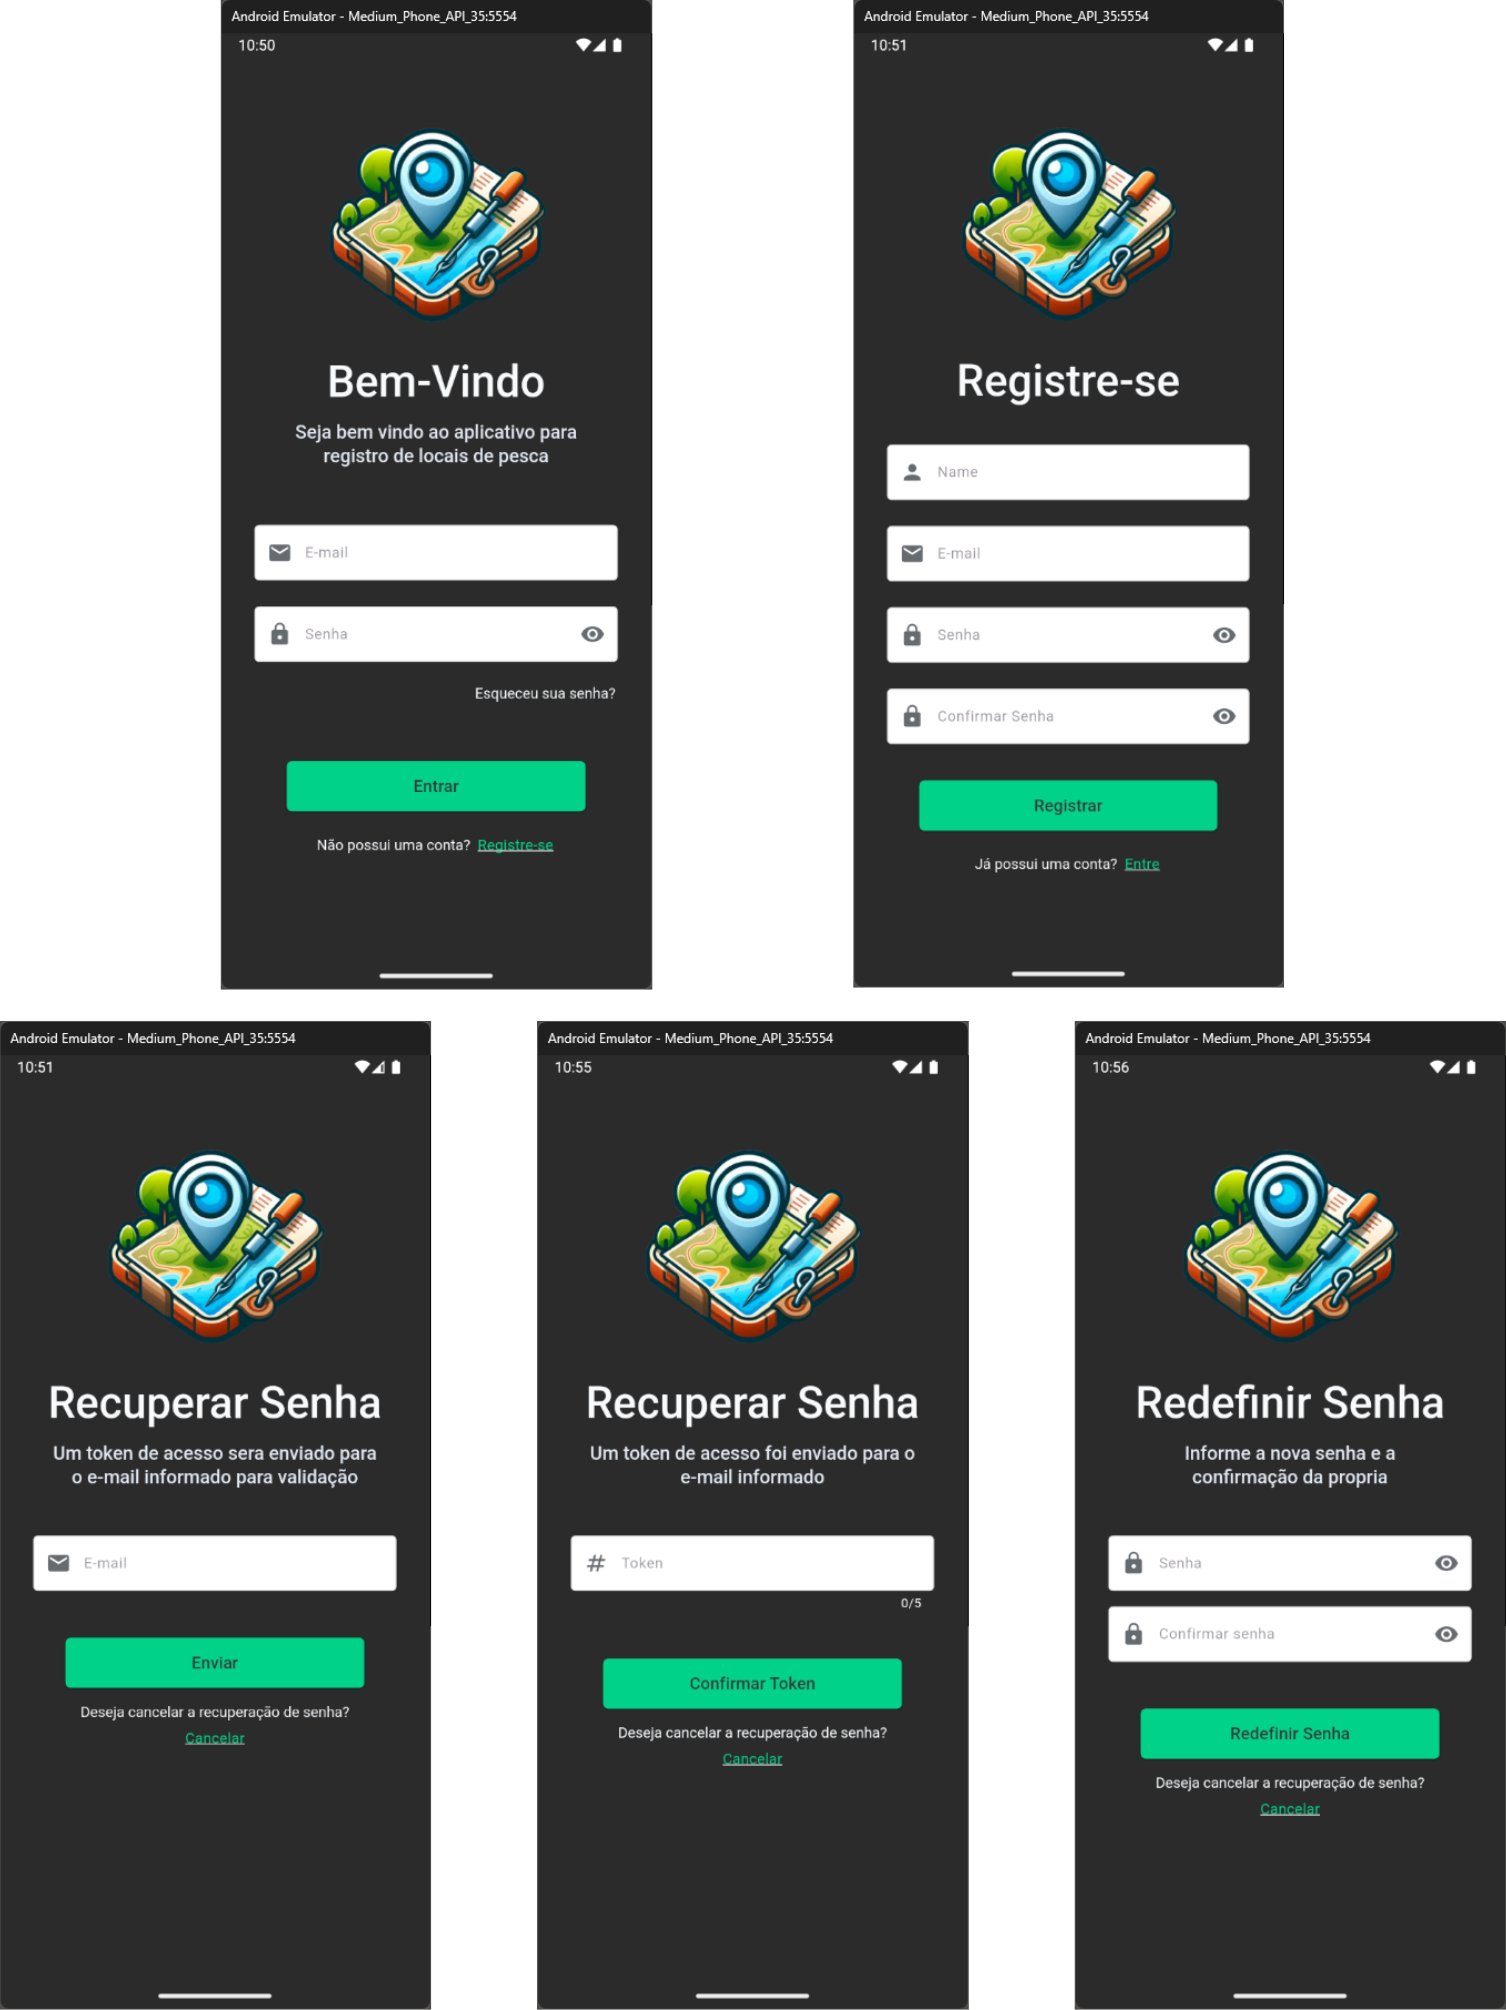
\includegraphics[scale=0.35]{./dados/figuras/emulator-auth-pages.png}
    \fonte{Produzido pelo Autor}
\end{figure}


As telas relacionadas ao mapa principal e aos detalhes dos usuário, tal qual um perfil de usuário, estão sendo representadas pela \autoref{fig:emultatorMapAndPerfilPages}. A figura mostra as páginas desenvolvidas no modo escuro, as quais proporcionam qualidade de observação duranto o uso do aplicativo para os usuários.

\begin{figure}[H]
    \centering
    \caption{Resultado Obtido - Telas de Mapa e Perfil}
    \label{fig:emultatorMapAndPerfilPages}
    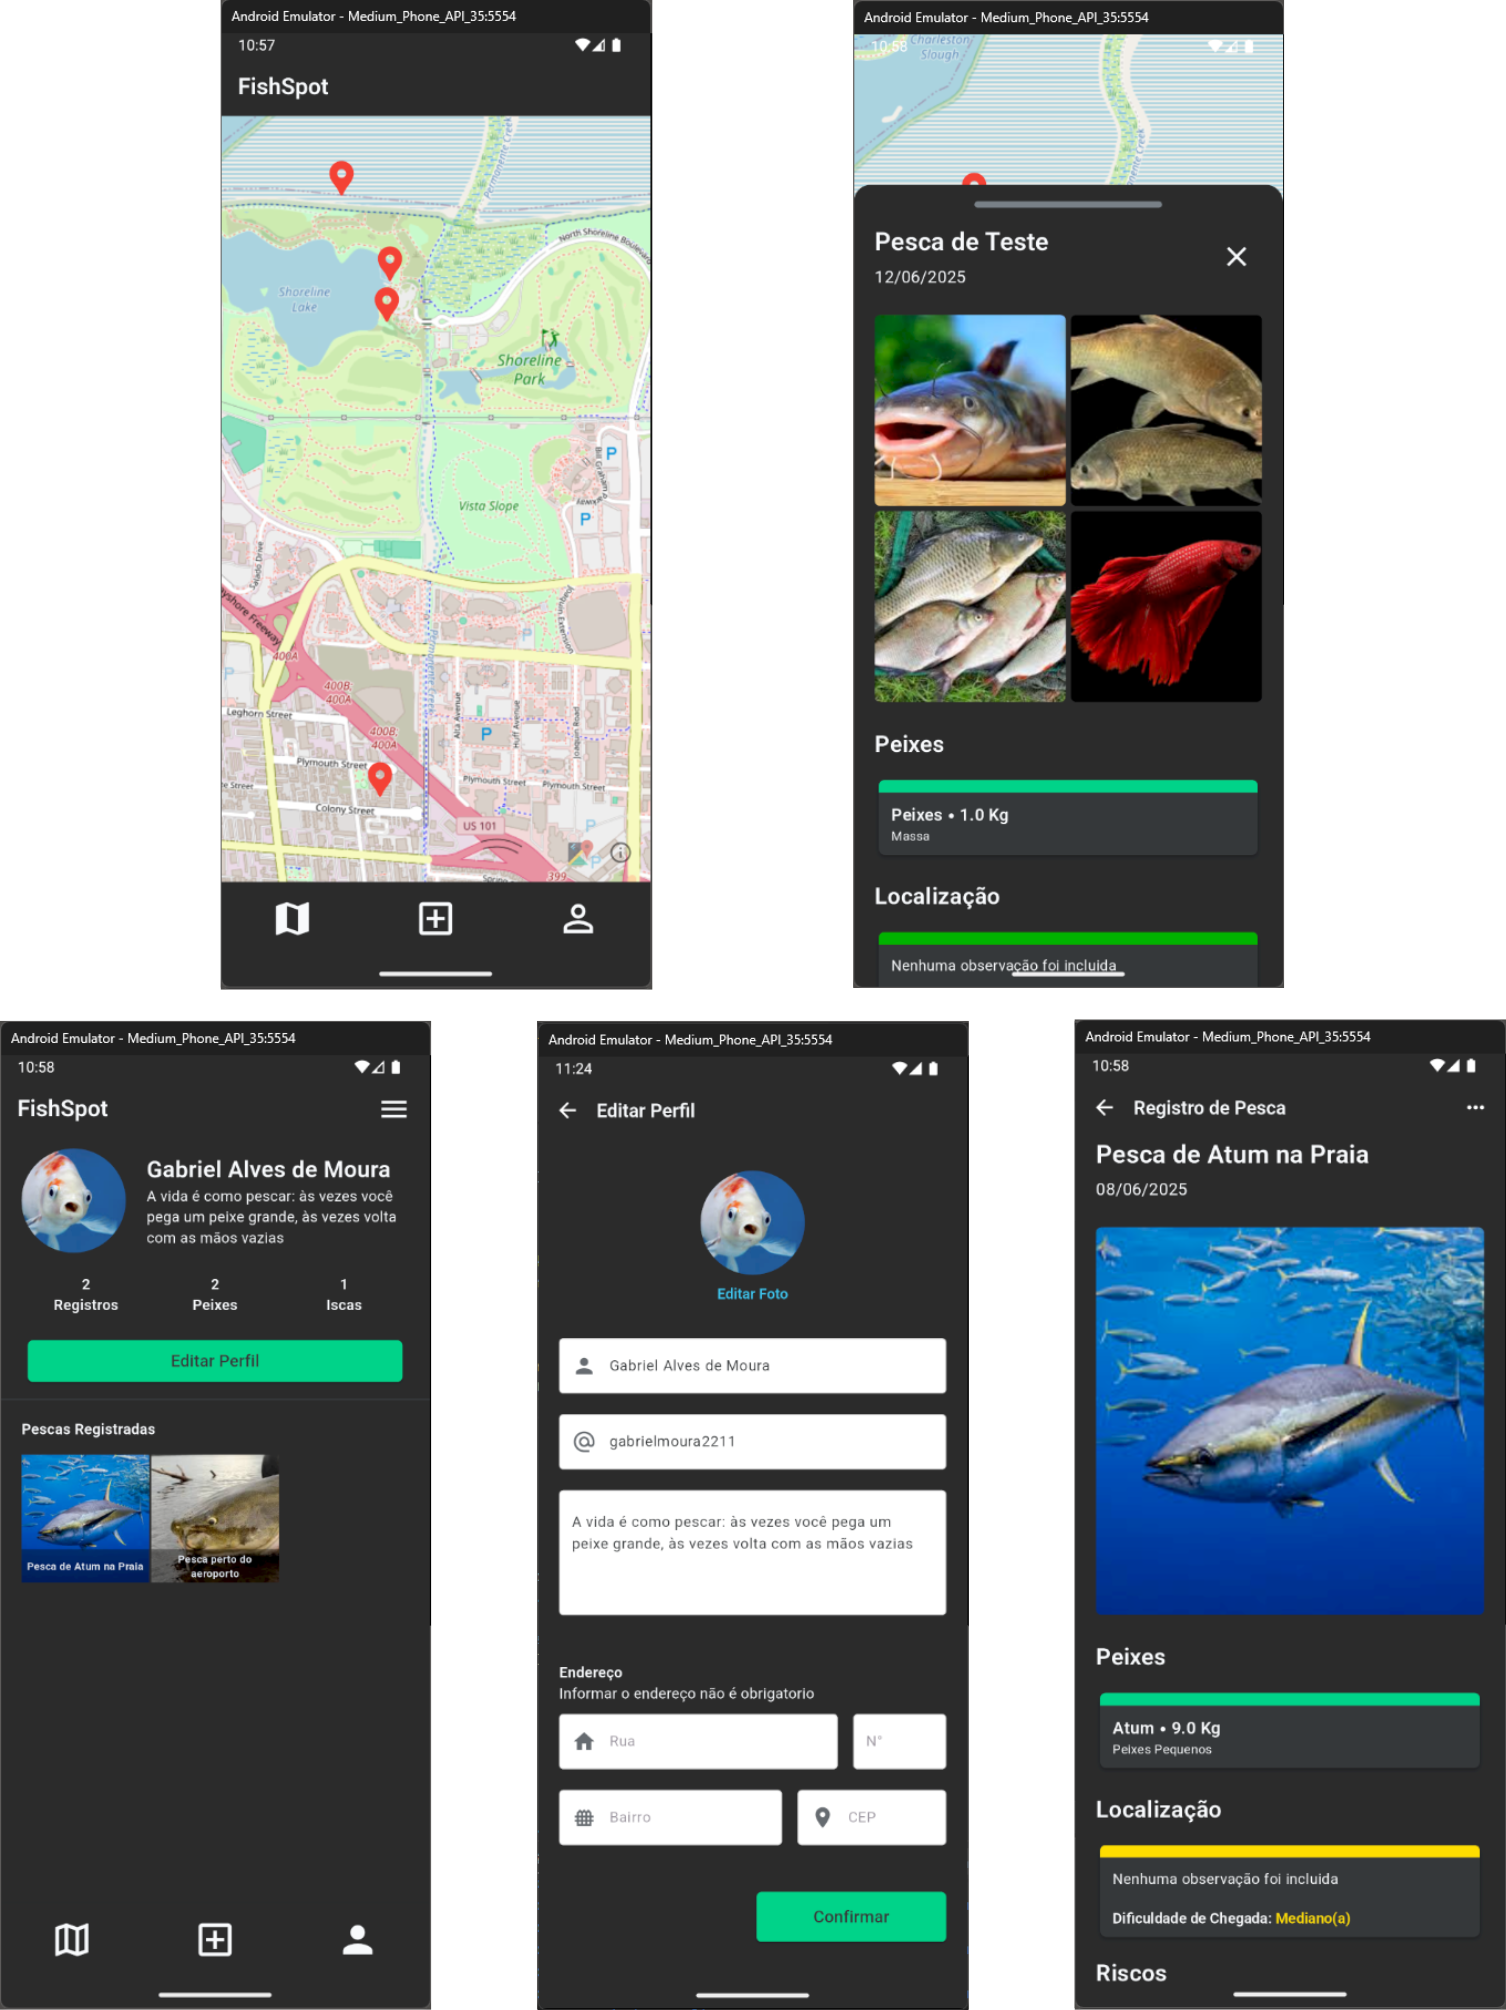
\includegraphics[scale=0.35]{./dados/figuras/emulator-map-and-profile-pages.png}
    \fonte{Produzido pelo Autor}
\end{figure}

O registro de um ponto de pesca está sendo representado pela \autoref{fig:emultatorSpotRegisterPages}, é possivel visualizar as páginas de severidade do local, inclusão de imagens, inclusão de espécies de peixes e descrição do ponto de pesca.

\begin{figure}[H]
    \centering
    \caption{Resultado Obtido - Telas de Registro de Ponto de Pesca}
    \label{fig:emultatorSpotRegisterPages}
    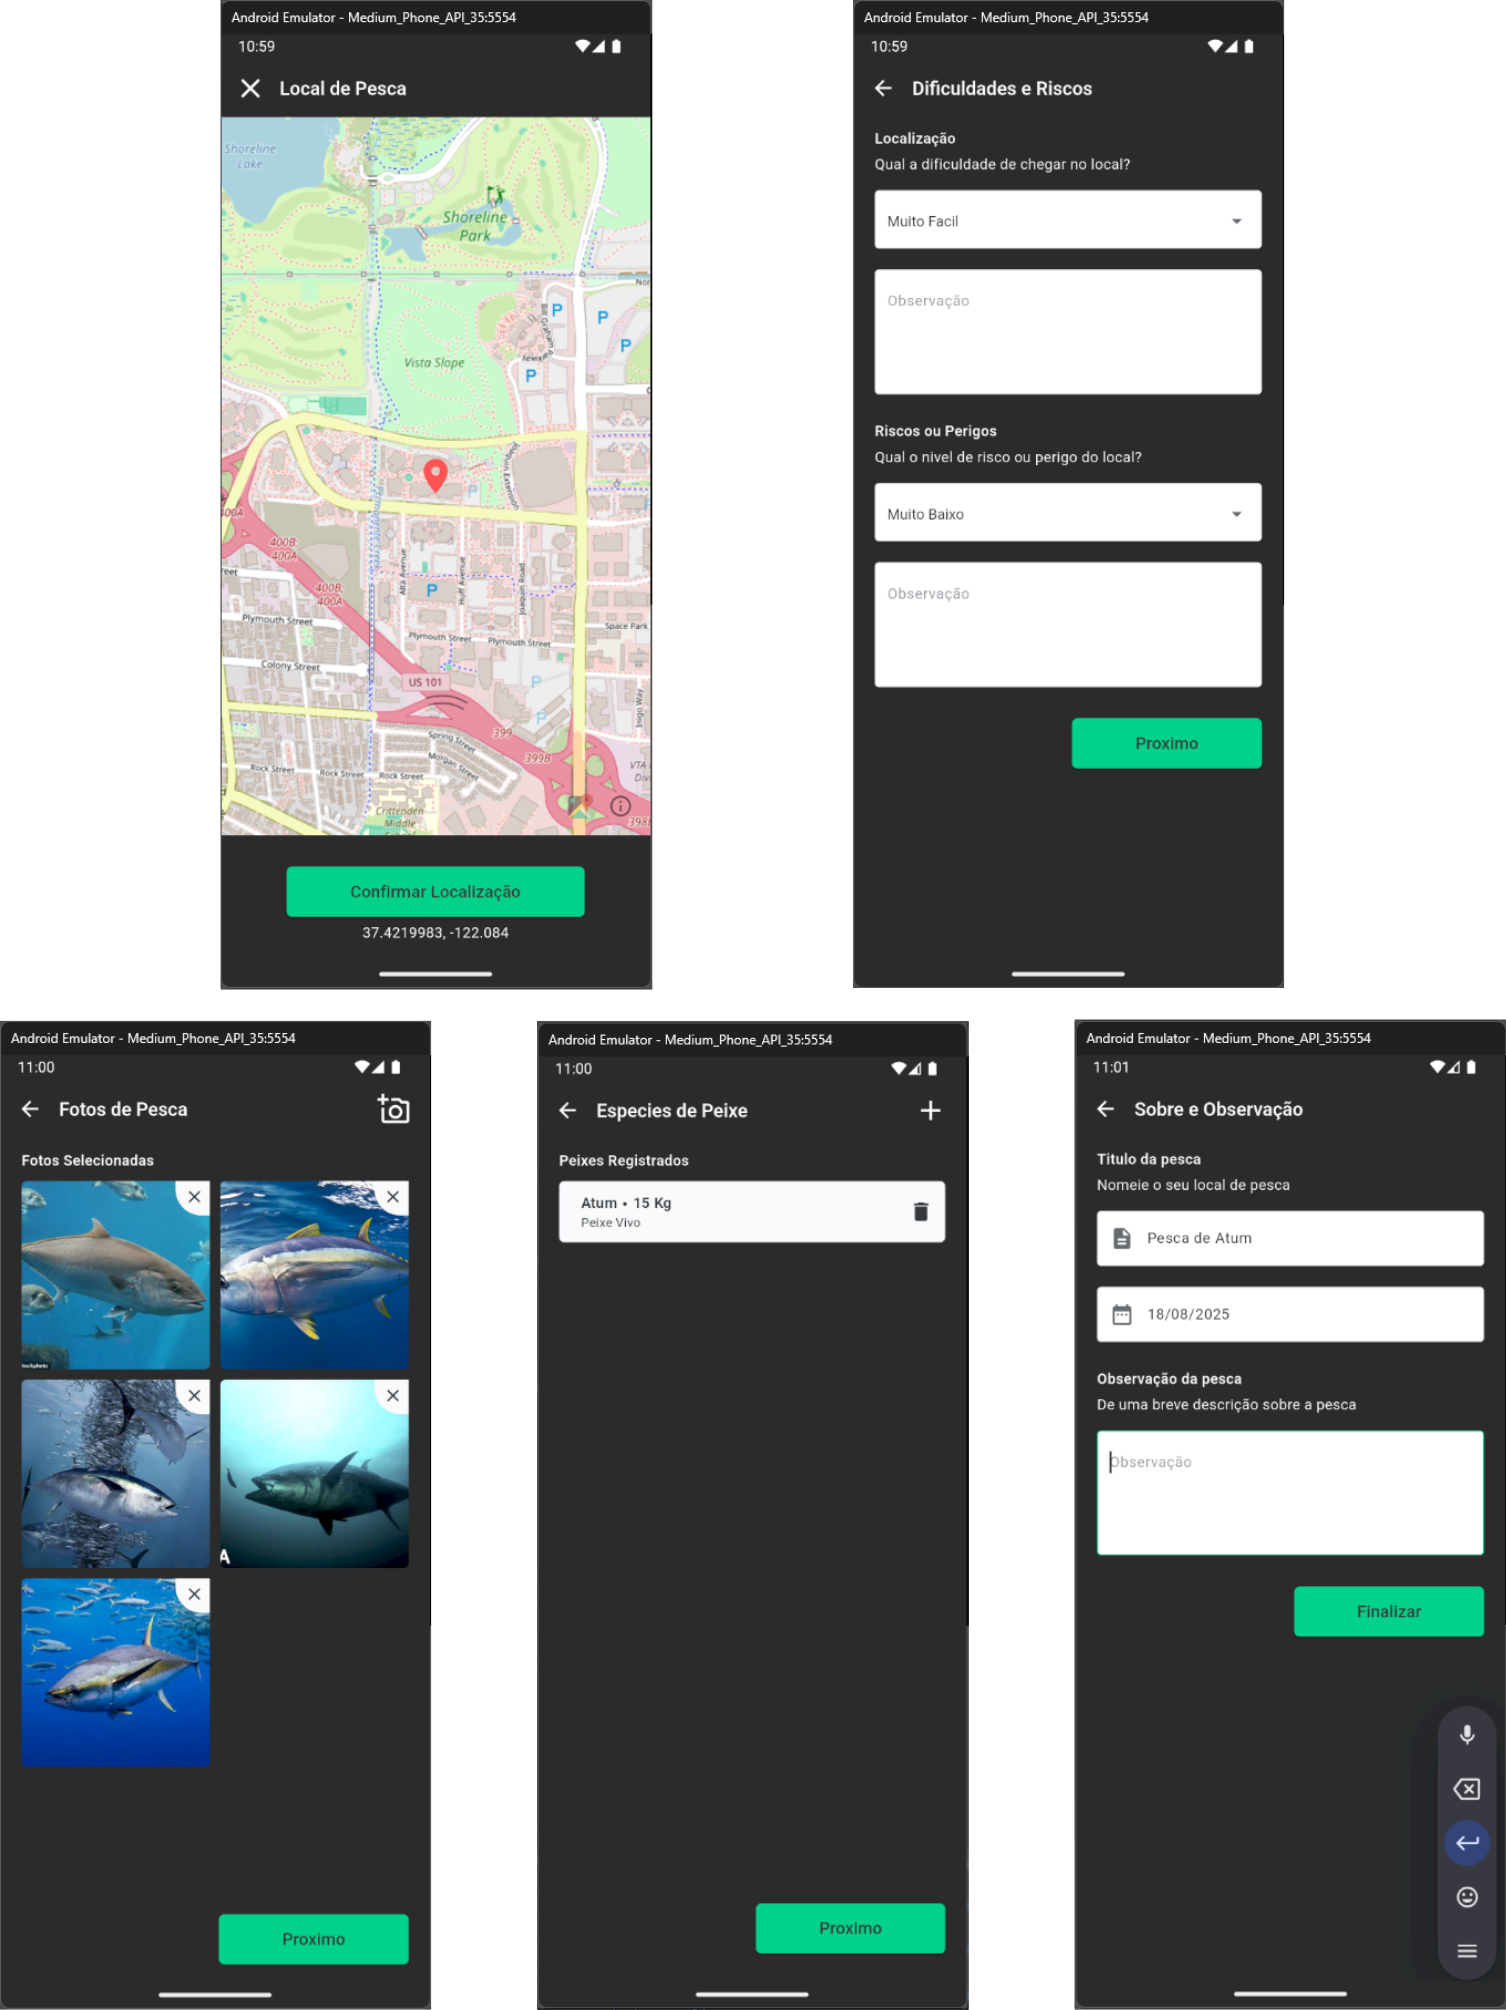
\includegraphics[scale=0.35]{./dados/figuras/emulator-spot-register-pages.png}
    \fonte{Produzido pelo Autor}
\end{figure}

% ---- Modo Claro

A \autoref{fig:emultatorAuthPagesLight} mostra as páginas relacionadas a autenticação do usuário, registro do usuário e recuperação de senha. Todas as telas foram desenvolvidas utilizando o esquema de cores do modo claro.

\begin{figure}[H]
    \centering
    \caption{Resultado Obtido - Telas de Autenticação}
    \label{fig:emultatorAuthPagesLight}
    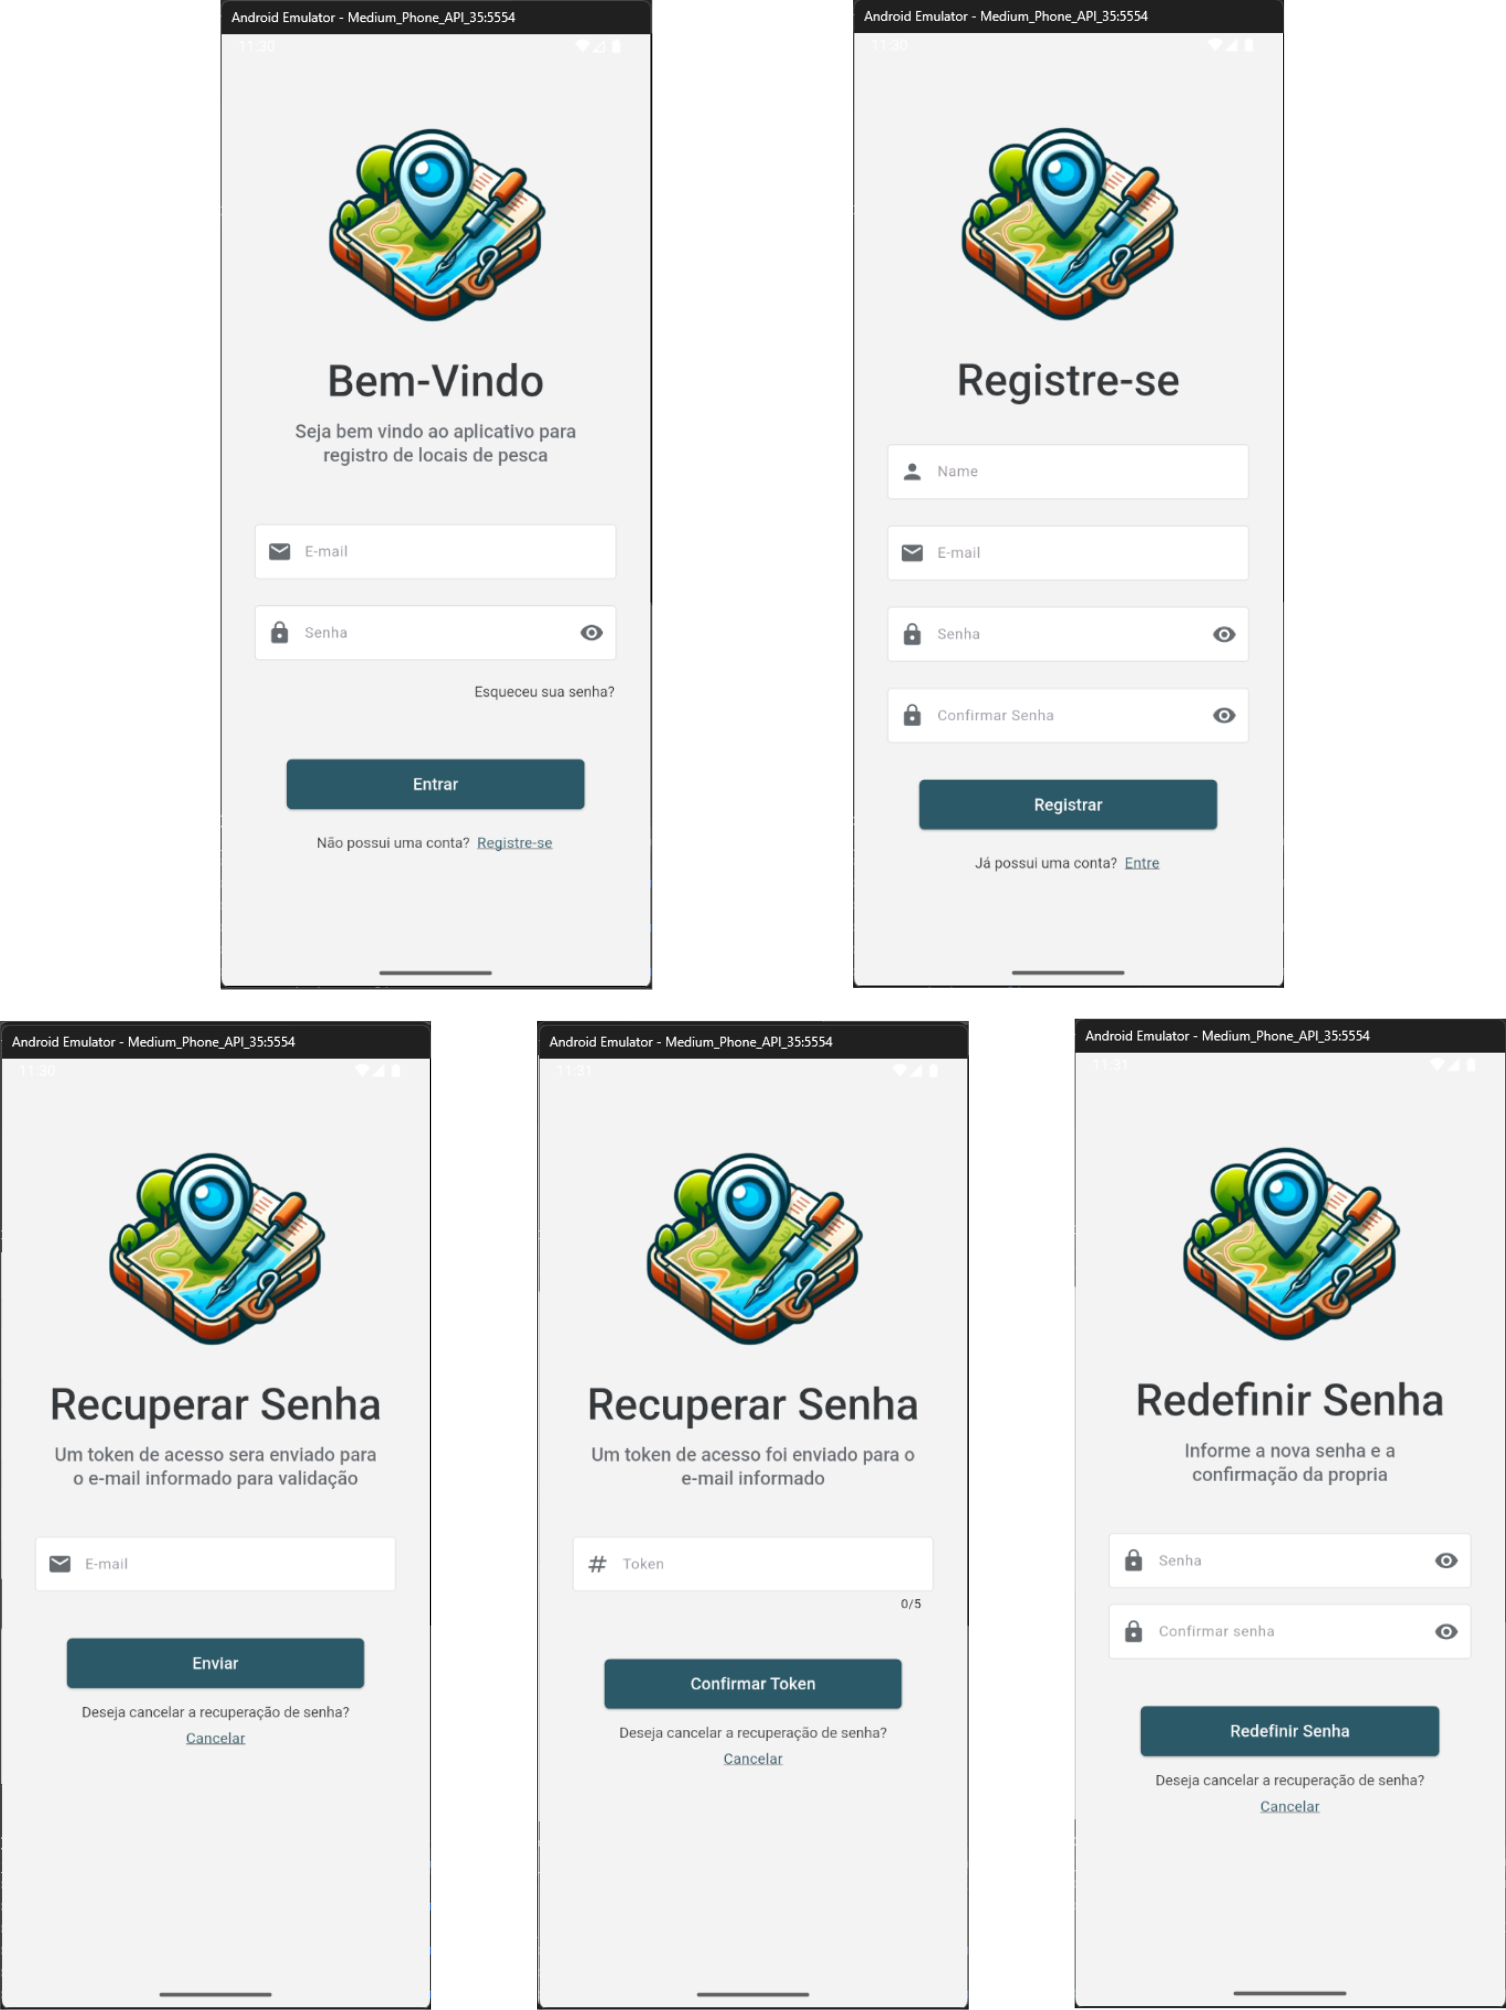
\includegraphics[scale=0.35]{./dados/figuras/emulator-auth-light-pages.png}
    \fonte{Produzido pelo Autor}
\end{figure}


Na \autoref{fig:emultatorMapAndPerfilPagesLight} é possível observar as telas relacionadas ao mapa princpial, detalhes do ponto de pesca, perfil do usuário e tambem edição dos dados do usuário, todas desenvolvidas utilizando esquema de cores do modo claro.

\begin{figure}[H]
    \centering
    \caption{Resultado Obtido - Telas de Mapa e Perfil}
    \label{fig:emultatorMapAndPerfilPagesLight}
    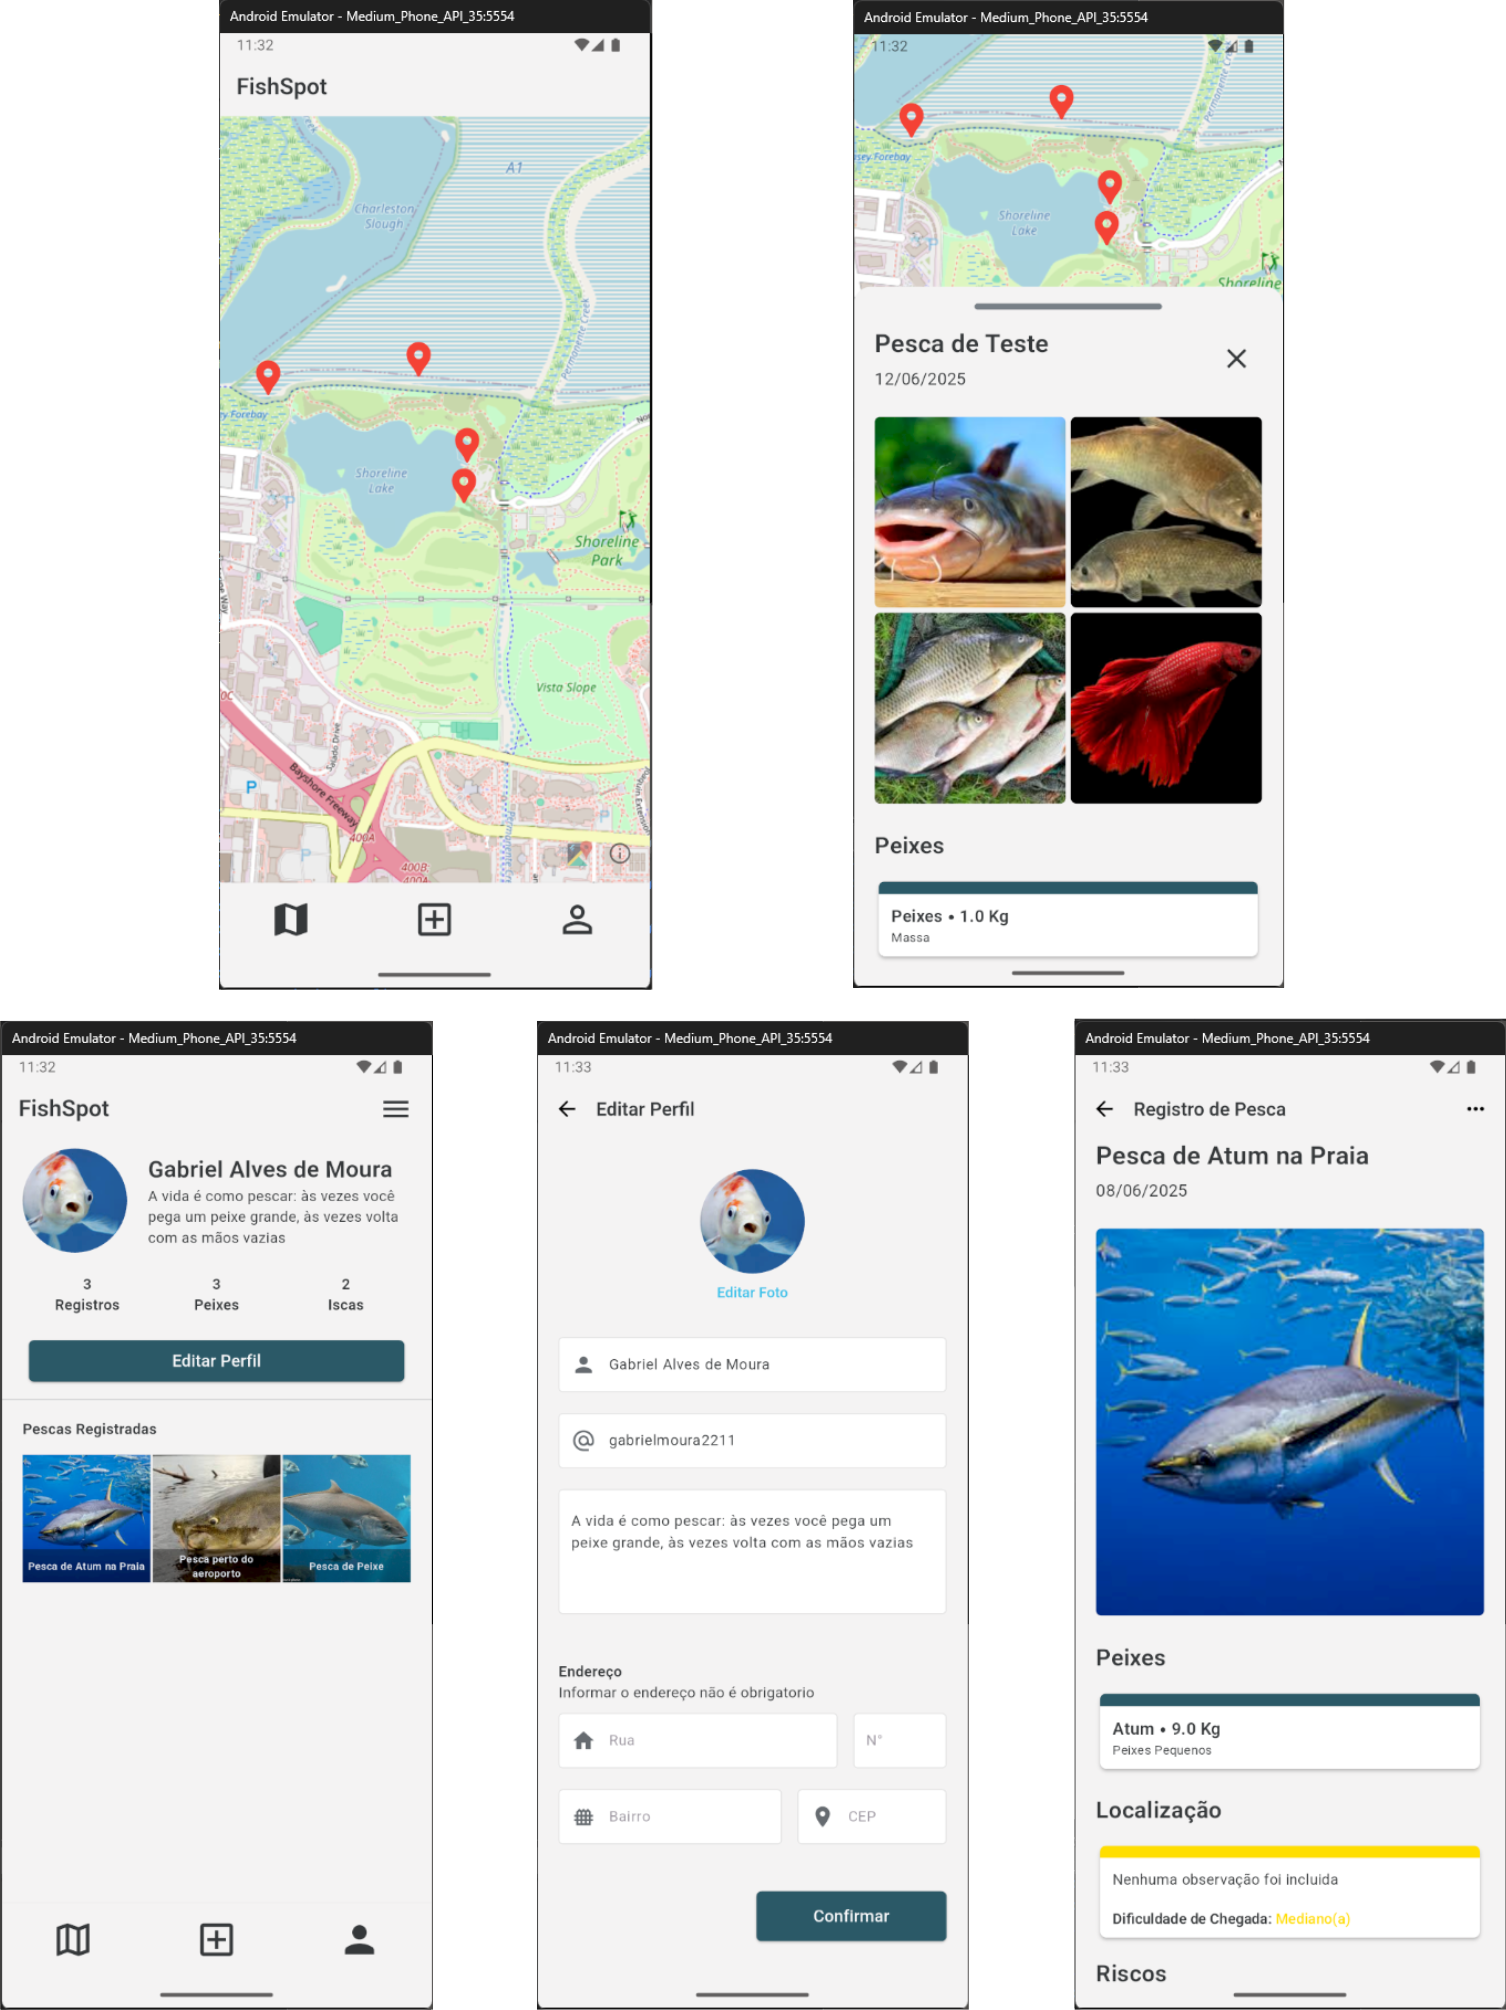
\includegraphics[scale=0.35]{./dados/figuras/emulator-map-and-profile-light-pages.png}
    \fonte{Produzido pelo Autor}
\end{figure}

O registro do ponto de pesca no modo claro está sendo apresentado pela \autoref{fig:emultatorSpotRegisterLightPages}, é possivel observar as telas de confirmação de geolocalização, severidade da localização, inclusão de imagens, inclusão de espécies de peixes e observação do ponto de pesca.

\begin{figure}[H]
    \centering
    \caption{Resultado Obtido - Telas de Registro de Ponto de Pesca}
    \label{fig:emultatorSpotRegisterLightPages}
    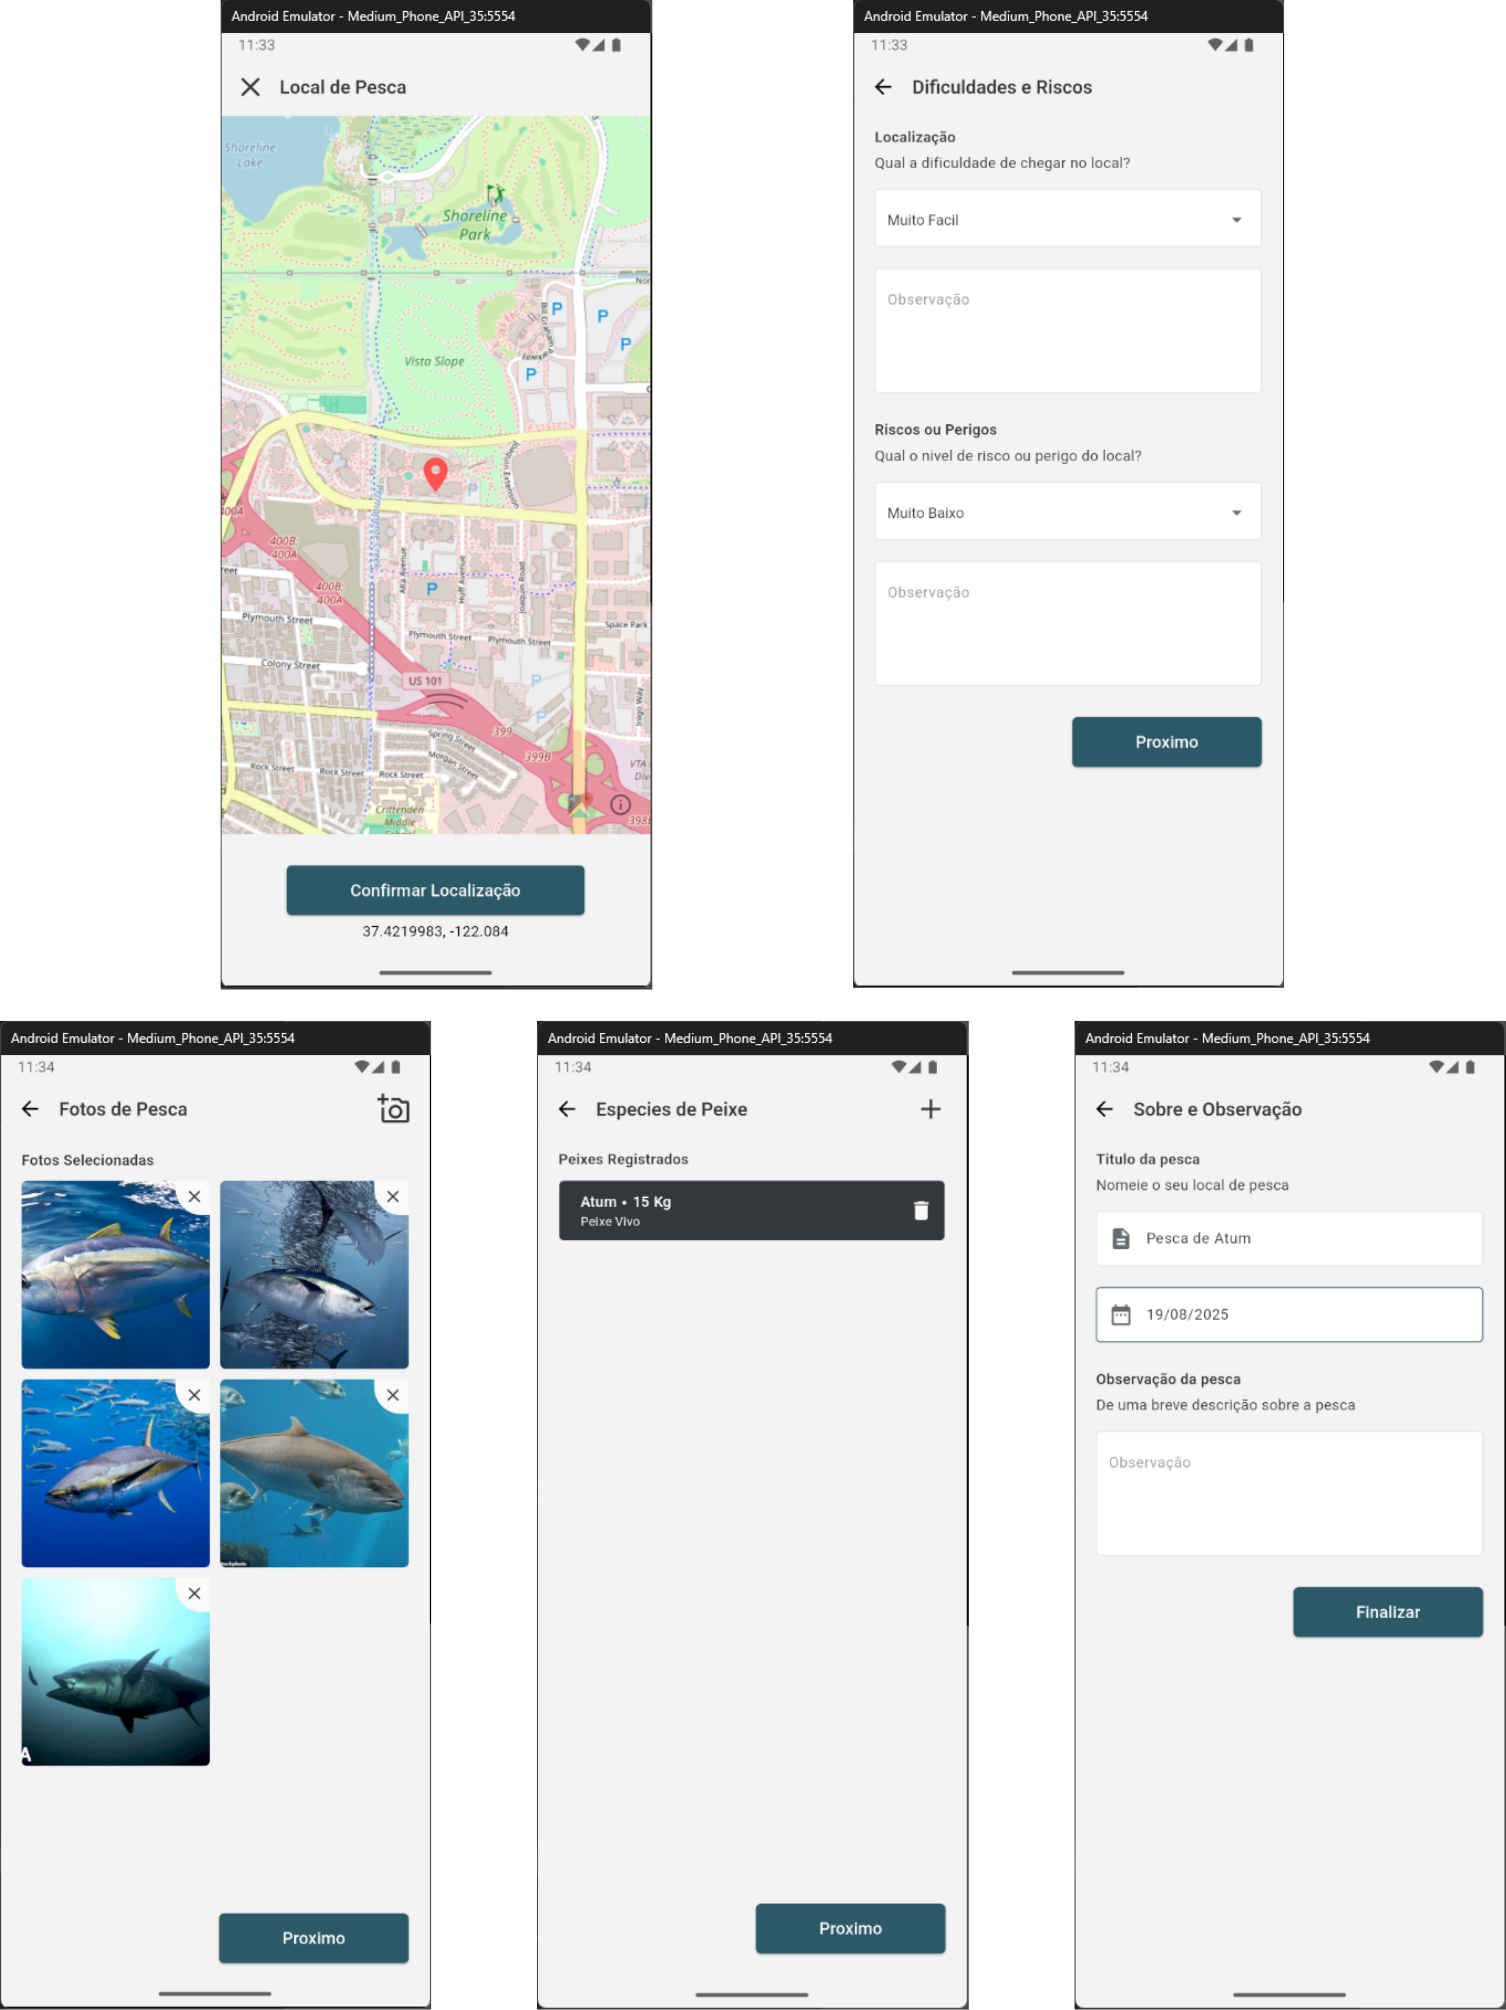
\includegraphics[scale=0.35]{./dados/figuras/emulator-spot-register-light-pages.png}
    \fonte{Produzido pelo Autor}
\end{figure}                                % Resultado
% CONCLUSÃO--------------------------------------------------------------------

\chapter{CONCLUSÃO}
\label{chap:conclusao}

                 			      % Conclusão

\postextual
% INSERE ELEMENTOS PÓS-TEXTUAIS
% REFERÊNCIAS------------------------------------------------------------------

% Carrega o arquivo "base-referencias.bib" e extrai automaticamente as referências citadas

\bibliography{./base-referencias}
\bibliographystyle{abntex2-alf} % Define o estilo ABNT para formatar a lista de referências
% OBSERVAÇÕES------------------------------------------------------------------
% Este arquivo não precisa ser alterado.
           			   % Referências
%% APÊNDICES--------------------------------------------------------------------

\begin{apendicesenv}
\partapendices

% Apêndice--------------------------------------------------------------------
\chapter{Nome do apêndice} % Edite para alterar o título deste apêndice
\label{chap:apendiceA}

\end{apendicesenv}
             			   % Apêndices
%% ANEXO------------------------------------------------------------------------

\begin{anexosenv}
\partanexos

% Primeiro anexo---------------------------------------------------------------
\chapter{Nome do anexo}     % edite para alterar o título deste anexo
\label{chap:anexoA}

\end{anexosenv}
               			   % Anexos

\end{document}
